%--------------------------------------
% Create title frame
\titleframe

%--------------------------------------
% Table of contents
\begin{frame}{Overview}
  \setbeamertemplate{section in toc}[sections numbered]
  \tableofcontents[hideallsubsections]
\end{frame}


\begin{frame} {Leçons précédentes}
\begin{itemize}
	\item Circuits linéaires, résistances, sources (commandées ou non) de courant et de tension.
	\item Lois de Kirchhoff
	\item Régime transitoire, éléments L et C.
	\item Régime sinusoïdal établi (RSE), notions de phaseurs et d'impédance (/admittance).
\end{itemize}
\vfill
\end{frame}

\begin{frame}{Qu'allons nous faire dans ce cours ?}
Nous analysons la notion de puissance en RSE. Nous établissons notamment la distinction entre les notions de \textbf{puissance active}, \textbf{réactive} et \textbf{apparente}, la notion de \textbf{facteur de puissance}, et caractérisons les dipôles R, L et C.
\vfill 
Nous introduisons la notion de circuits magnétiquement couplés, ce qui mène à la notion de \textbf{transformateur}, quadripôle omniprésent dans les circuits et réseaux électriques pour adapter les niveaux de tension, de courant, etc. entre différents circuits.
\vfill 	
Finalement, nous introduisons le concept de \textbf{triphasé}, très utilisé en transport et distribution de l'énergie électrique.
\vfill 

\textbf{Dans le syllabus :} le reste du chapire 4, tous les exercices du chapitre 4 mais plus précisément les exercices 4.6 à 4.15.

\end{frame}

%-----------------------------------------------------------------------------------

\section{Exemple illustratif}

\begin{frame}{Énoncé et Données}

Un circuit RL série est alimenté par une source de tension sinusoïdale de valeur efficace $V_{eff} = 230 \, \text{V}$ et de fréquence $f = 50 \, \text{Hz}$. Le circuit est composé de :
\begin{itemize}
    \item Une résistance $R = 10 \, \Omega$
    \item Une inductance $L = 100 \, \text{mH}$
\end{itemize}

\begin{block}{Exercice}
Dessinez le circuit. 
\end{block}

\alert{Question: quel courant circule dans le circuit ?}
\end{frame}

\begin{frame}{Analyse de l'Impédance}

La pulsation du signal est donnée par :
\[ \omega = 2\pi f = 2\pi \cdot 50 = 100\pi \approx 314,16 \, \text{rad/s} \]
L'impédance complexe totale $Z_{eq}$ du circuit série est :
\[ Z_{eq} = R + jL\omega = 10 + j(0,1 \cdot 100\pi) = 10 + j31,4 \, \Omega \]


\textbf{Forme polaire :}
\begin{itemize}
    \item Module : $|Z_{eq}| = \sqrt{R^2 + (L\omega)^2} = \sqrt{10^2 + 31,4^2} \approx 32,95 \, \Omega$
    \item Phase (déphasage) : $\phi = \arctan\left(\frac{L\omega}{R}\right) = \arctan\left(\frac{31,4}{10}\right) \approx 72,3^\circ$
\end{itemize}
\end{frame}

\begin{frame}{Calcul de l'Intensité}
En prenant la tension comme référence de phase ($\bar{V} = 230e^{j0}$), l'intensité complexe est :
\[ \bar{I} = \frac{\bar{V}}{Z_{eq}} = \frac{230}{32,95e^{j72,3^\circ}} \approx 6,98 e^{-j72,3^\circ} \, \text{A} \]
La valeur efficace du courant est donc $I_{eff} \approx 6,98 \, \text{A}$.

\begin{block}{Questions:}
\begin{itemize}
	\item quelle est la puissance consommée par la résistance ?
	\item quelle est la puissance totale consommée par le circuit RL ?
	 \item comment ceci évoluerait-il si $L$ était plus faible, tout le reste étant inchangé ? 
\end{itemize}	
\end{block}



\end{frame}

\section{Puissances en régime sinusoïdal établi}
\subsection{Domaine temporel}

\begin{frame}{Rappel : formules de Simpson}
\begin{itemize}
\item $\cos(a+b) = \cos(a)\cos(b)-\sin(a)\sin(b)$
\item $\cos(a-b) = \cos(a)\cos(b)+\sin(a)\sin(b)$
\item $\cos(a) \cos(b) = \frac{1}{2} \left(\cos(a-b)+\cos(a+b)\right)$
\end{itemize}
\end{frame}

\begin{frame}{Puissance instantanée}
	
	\begin{columns}
		\begin{column}{0.3\linewidth}
		\centering
		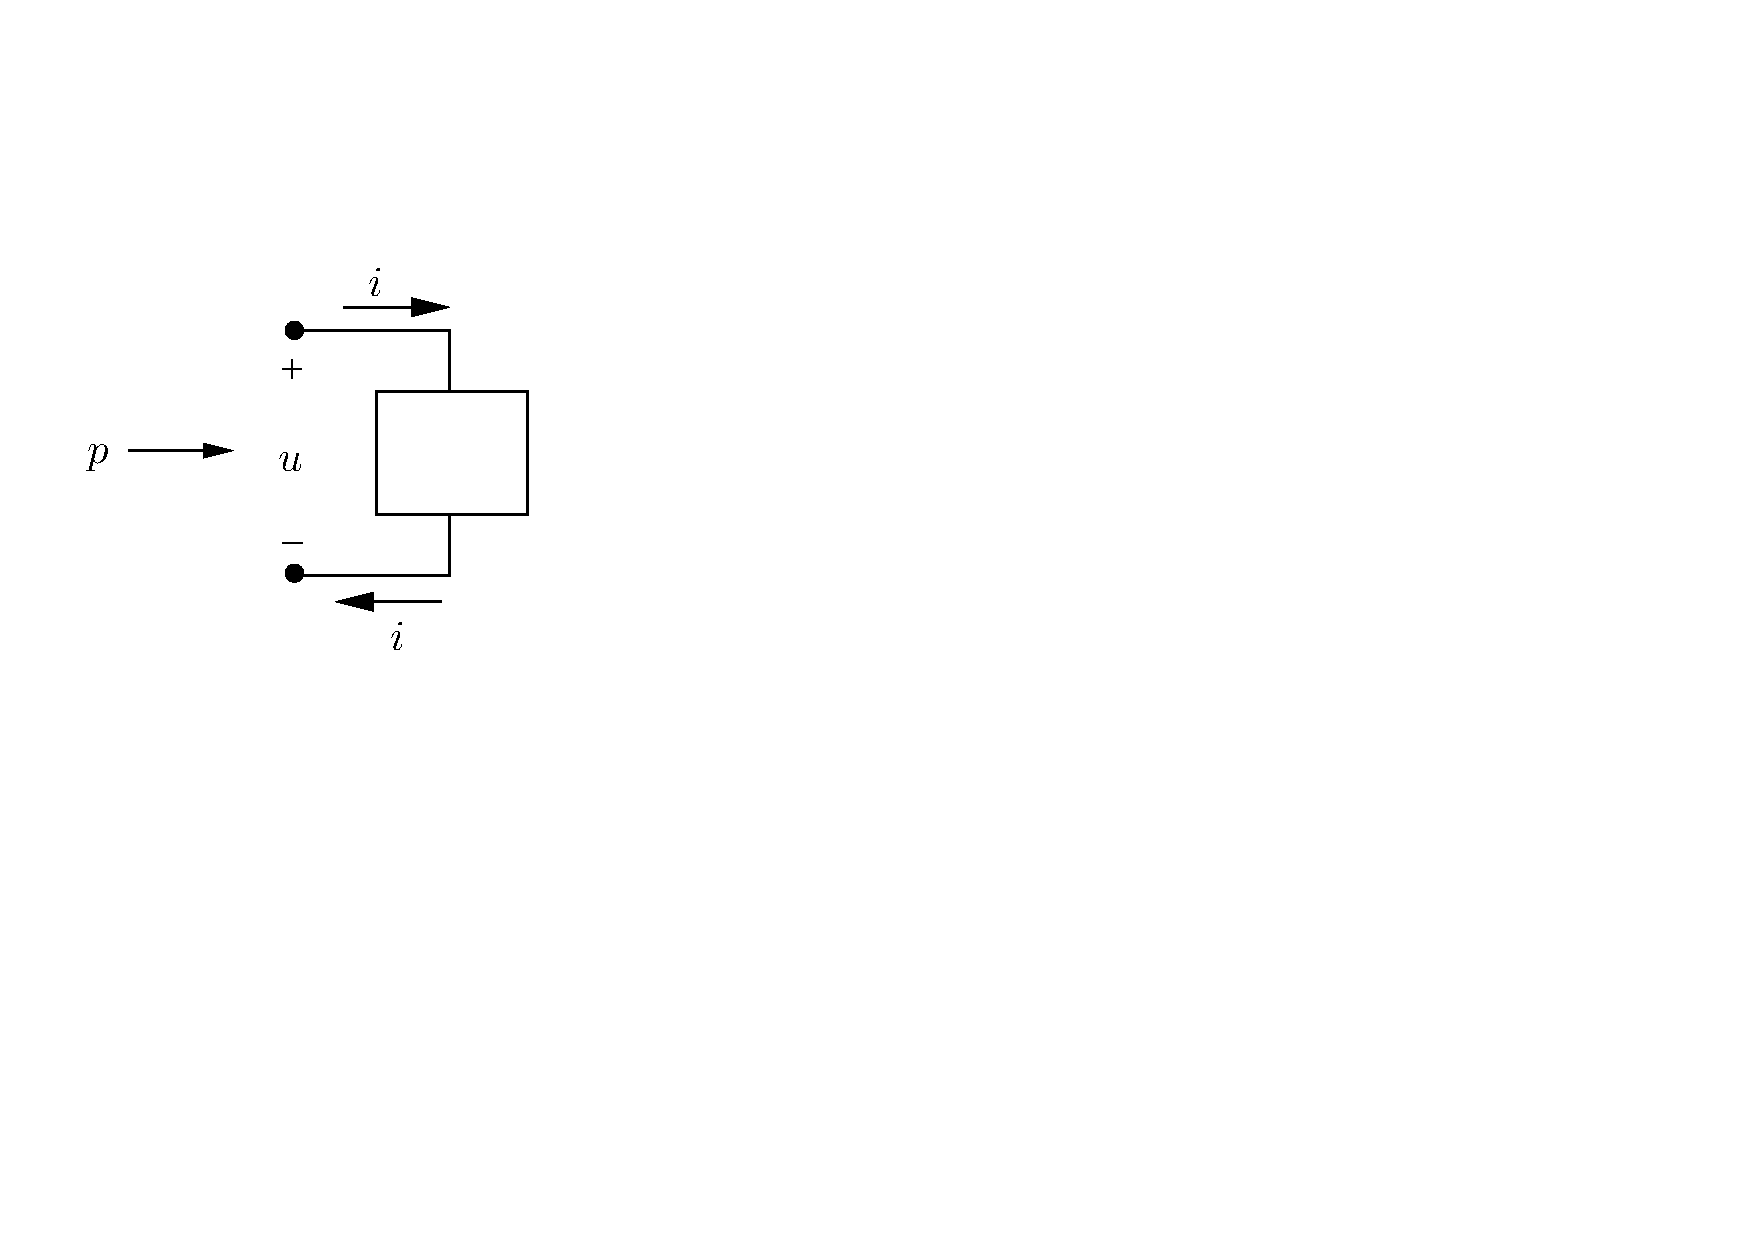
\includegraphics[width=0.8\linewidth]{dipole}
		\end{column}
		\begin{column}{0.68\linewidth}
			{\small\[
				u(t)=U_m\cos(\omega t + \phi_u) \qquad i(t)=I_m\cos(\omega t + \phi_i)\]}
			Puissance {\em instantanée~} fournie au dipôle :
			{\small \begin{eqnarray*}
					p(t)& = &u(t)i(t)\\ & =&U_mI_m\cos(\omega t + \phi_u)\cos(\omega t +\phi_i) \\
					& = & \frac{1}{2}U_mI_m\left[\cos(\phi_u-\phi_i)+\cos(2\omega t+\phi_u+\phi_i)\right]
				\end{eqnarray*}}
			\end{column}
		\end{columns}
		
		En utilisant les valeurs efficaces :
		 \[U=\frac{U_m}{\sqrt{2}} \qquad I=\frac{I_m}{\sqrt{2}}\]
			
		\begin{block}{Puissance instantanée}
			$$p(t) = U\,I\left[\cos(\phi_u-\phi_i)+\cos(2\omega t+\phi_u+\phi_i)\right]$$
		\end{block}
	\end{frame}
	
	
	%-----------------------------------------------------------------------------------
	
	\begin{frame}{Puissance instantanée}
		\begin{columns}
		\begin{column}{0.45\textwidth}
			La puissance instantanée $p(t)$
			\begin{itemize}
				\item oscille à une fréquence double de celle de $u$ et $i$
				\item est alternativement positive et négative $\rightarrow$ échanges d'énergie 
			\end{itemize}		
		\end{column}
		\begin{column}{0.45\textwidth}
			\begin{center}
				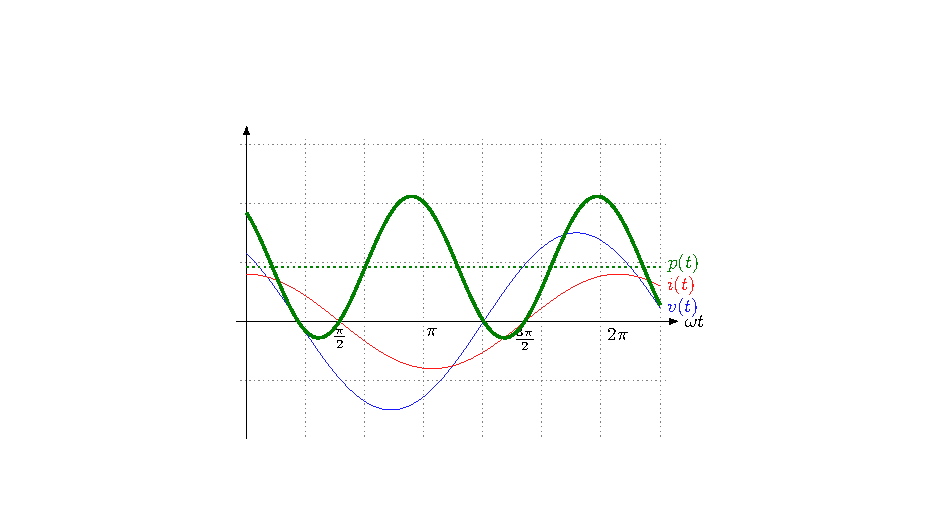
\includegraphics[width=\textwidth]{dephasage_U_I_et_P.pdf}
				%\PowerTimeDiagram{40}{1.5}{0.8}
			\end{center}
		\end{column}
		\end{columns}
	\end{frame}
	
	\begin{frame}[allowframebreaks]{La puissance instantanée $p(t) = P + p_f(t)$ }
		

		\begin{block}{Puissance active}
		Le terme constant $P=U\,I\cos(\phi_u-\phi_i)$
		\begin{itemize}
			\item représente la puissance moyenne fournie au dipôle par période,
			et donc la puissance réellement utilisable 
			{\small \[P=\frac{1}{T}\int_0^T p(t)\, dt\]}
			\item dépend de l'\textbf{amplitude} de $u$ et $i$ \textbf{\underline{et}} de
			leur \textbf{déphasage} $\phi_u-\phi_i$
			\item $P$ est appelée {\em puissance active}
		\end{itemize}
		\end{block}
		
		\begin{block}{Puissance fluctuante}
		Le terme oscillant $p_f=U\,I\cos(2\omega t+\phi_u+\phi_i)$
		\begin{itemize}
			\item est appelé puissance fluctuante;
			\item est de moyenne nulle;
		\end{itemize}
		\end{block}
	\end{frame}
	
	%-----------------------------------------------------------------------------------
	
	\begin{frame}{Puissance réactive}
		On a $p(t)=P+p_f(t)$. En réécrivant $p_f(t)$, on obtient
		\begin{align*}
			p_f(t)& = U\,I\cos (2(\omega t + \phi_u)-(\phi_u-\phi_i))\\
			& = P \cos 2(\omega t+\phi_u) + Q \sin 2(\omega t+\phi_u)
		\end{align*}
		
		\begin{block}{Puissance réactive}
		\[Q = U\,I\sin (\phi_u-\phi_i)\]

		
		Elle est due au déphasage existant
		entre $u$ et $i$ et est liée aux échanges d'énergie magnétique et
		électrostatique survenant dans le circuit suite à la présence
		d'inductances et de condensateurs. 
		\end{block}
		


	\end{frame}
	
	\begin{frame}{Puissance apparente}
	\begin{block}{Puissance apparente}
		Le produit $U\,I$ est appelé {\em puissance apparente}.
	\end{block}	

	\vfill
	
	Wikipedia: \textit{"Electrical engineers \textbf{take apparent power into account} when designing and operating power systems, because though the current associated with reactive power does no work at the load, it heats the conductors and wastes energy. \textbf{Conductors, transformers and generators must be sized to carry the total current, not just the current that does useful work}."}
	\end{frame}
	
	\begin{frame}{Unités}
		Pour distinguer ces différents types de puissance, on les exprime dans des unités spécifiques.
		\begin{block}{Unités}
			\begin{itemize}
				\item $p(t)$, $p_f(t)$, $P$ : W
				\item $Q$ : var (volt.ampère réactif)
				\item puissance apparente : VA (volt.ampère)
			\end{itemize}
		\end{block}
	\end{frame}

	%-----------------------------------------------------------------------------------
	\subsection{Calculs dans le domaine fréquentiel}
	\begin{frame}{Domaine fréquentiel}
		
		On peut calculer les puissances active, réactive et apparente à partir des phaseurs. 
		
		\begin{block}{Puissance complexe}
		La puissance complexe est obtenue en formant le produit \alert{hermitique} :
		\begin{eqnarray*}
			S&=&\bar{U}\bar{I}^{\mathcolor{orange}{*}}\\
			& = & Ue^{j\phi_u}\,Ie^{{\mathcolor{orange}{-}}j\phi_i}= U\, Ie^{j(\phi_u-\phi_i)}\\
			& = & U\,I \left(\cos(\phi_u-\phi_i)+j\sin(\phi_u-\phi_i)\right)\\
			& = & P + j Q			
		\end{eqnarray*}
	\end{block}
	
	La puissance apparente est le module de la puissance complexe:
	$$|S|=U\,I=\sqrt{P^2+Q^2}.$$

	\end{frame}
	
\subsection{Propriétés des impédances de dipôles RLC passifs}	
	\begin{frame}{Dipôle purement résistif}
		$u$ et $i$ sont en phase : $\phi_u-\phi_i=0$
		
		\begin{eqnarray*}
			p(t)& = &u(t)i(t)=RI_m^2\cos^2(\omega t + \phi_u)\\
			& =& RI^2(1+\cos 2(\omega t + \phi_u))\\
			& = & P + P \cos 2(\omega t+ \phi_u)
		\end{eqnarray*}
		
		\begin{itemize}
		\item $p$ toujours positif !
		\item de moyenne $P=RI^2$
		\item $p_f= P \cos 2(\omega t+ \phi_u)$
		\item $Q=0$ !
		\end{itemize}

	\end{frame}
	
	%-----------------------------------------------------------------------------------
	

	\begin{frame}{Dipôle purement inductif}
		
		$i$ est en retard de 90$^{\circ}$ par rapport à $u$ :
		$\phi_u-\phi_i=90^{\circ}$
		
		\begin{eqnarray*}
			p(t)& =& \omega L I_m^2 \cos(\omega t+\phi_u)\cos (\omega
			t+\phi_u - 90^{\circ})\\
			& = & \omega L\, I^2 \sin (2(\omega t + \phi_u))\\
			& = & Q \sin (2(\omega t + \phi_u))
		\end{eqnarray*}
		
		\begin{itemize}
		\item $p$ de moyenne nulle $\rightarrow P=0$ !\\
		\item $p_f= Q \sin 2(\omega t+ \phi_u)$
		\item $Q=\omega L\, I^2$
		\item Echanges périodiques d'énergie entre les inductances et le reste du circuit.
		\item Une inductance consomme de la puissance réactive  
		\end{itemize}
	\end{frame}
	
	%-----------------------------------------------------------------------------------
	
	\begin{frame}{}
		Dans un circuit purement inductif, la puissance instantanée oscille
		deux fois par période entre $-\omega L I^2$ et $\omega L I^2$.
		
		L'énergie magnétique stockée à l'instant $t$ dans l'inductance est :
		\[w_L(t)= \frac{1}{2}Li^2(t)=\frac{1}{2} L I^2(1+\cos (2(\omega
		t + \phi_i)) \geq 0 !\]
		
		L'énergie magnétique moyenne par période est
		
		\[<W_m>=\frac{1}{2}LI^2\]
		
		On a la relation entre la puissance réactive consommée par
		l'inductance et l'énergie magnétique
		moyenne : 
		\[ Q = 2\omega <W_m>\]
	\end{frame}
	
	%-----------------------------------------------------------------------------------
	
	\begin{frame}{Dipôle purement capacitif}
		
		$i$ est en avance de 90$^{\circ}$ par rapport à $u$ :
		$\phi_u-\phi_i=-90^{\circ}$
		
		\begin{eqnarray*}
			p(t)& = &\omega C U_m^2 \cos(\omega t+\phi_u)\cos (\omega
			t+\phi_u + 90^{\circ})\\
			& = & -\omega C\, U^2 \sin (2(\omega t + \phi_u))\\
			& = & Q \sin (2(\omega t + \phi_u))
		\end{eqnarray*}
		
		\begin{itemize}
		\item $p$  de moyenne nulle  $\rightarrow P=0$ !
		\item $p_f= Q \sin 2(\omega t+ \phi_u)$
		\item $Q=-\omega C\, U^2$
		\item Echanges périodiques d'énergie entre les condensateurs et le reste du circuit.
		\item Un condensateur produit de la puissance réactive 
		\end{itemize}

	\end{frame}
	
	%-----------------------------------------------------------------------------------
	
	\begin{frame}{}
		Dans un circuit purement capacitif, la puissance instantanée oscille
		deux fois par période entre $-\omega C U^2$ et $\omega C U^2$.
		
		L'énergie électrostatique  stockée à l'instant $t$ dans le condensateur est :
		\[w_C(t)= \frac{1}{2}Cu^2(t)=\frac{1}{2} C U^2(1+\cos (2(\omega
		t + \phi_u)) \geq 0 !\]
		
		L'énergie électrostatique  moyenne par période est
		
		\[<W_e>=\frac{1}{2}CU^2\]
		
		On a la relation entre la puissance réactive fournie par le condensateur
		et l'énergie électrostatique moyenne :
		\[ Q = - 2\omega <W_e>\]
	\end{frame}
	
	%-----------------------------------------------------------------------------------
	
	\begin{frame} {Résumé}	
		\begin{center}
			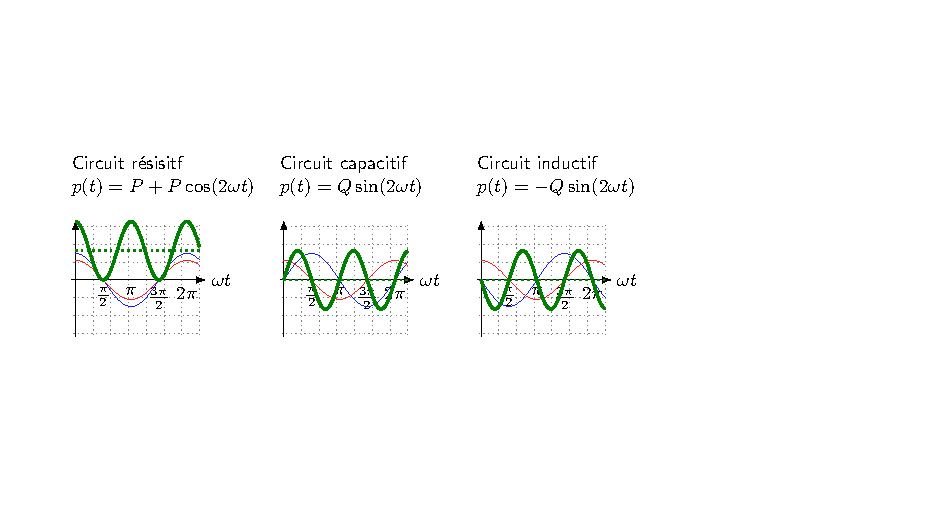
\includegraphics[width=\textwidth]{RLC_dephasage_U_I.pdf}
		\end{center}
		%\begin{tabular}{l l l}
			%Circuit  résisitf& Circuit capacitif & Circuit inductif\\
			%$p(t)= P + P\cos(2\omega t)$ & $p(t)=Q\sin(2\omega t)$ & $p(t)= - Q\sin(2\omega t)$\\
			%\PowerTimeDiagramR{1.5}{1.1} & \PowerTimeDiagramC{1.5}{1.1} & \PowerTimeDiagramL{1.5}{1.1} \\
		%\end{tabular}
	\end{frame}

	\begin{frame}[allowframebreaks]{Revenons à notre exemple : Bilan des Puissances}
	La puissance complexe $S$ est obtenue par le produit de la tension et du complexe conjugué de l'intensité :
	\[ {S} = \bar{V} \cdot \bar{I}^* = 230 \cdot 6,98e^{+j72,3^\circ} \]
	\[ {S} \approx 1605,4e^{j72,3^\circ} \, \text{VA} \]

	En utilisant la forme rectangulaire ${S} = P + jQ$ :
	\begin{itemize}
		\item \textbf{Puissance active :} $P = \text{Re}({S}) = 1605,4 \cdot \cos(72,3^\circ) \approx 487 \, \text{W}$
		\item \textbf{Puissance réactive :} $Q = \text{Im}({S}) = 1605,4 \cdot \sin(72,3^\circ) \approx 1529 \, \text{var}$
	\end{itemize}

	Synthèse des Résultats:
	\begin{table}[h]
		\centering
		\begin{tabular}{lcr}
			\toprule
			Grandeur & Symbole & Valeur \\
			\midrule
			Impédance totale & $|Z_{eq}|$ & $32,95 \, \Omega$ \\
			Courant efficace & $I_{eff}$ & $6,98 \, \text{A}$ \\
			%Facteur de puissance & $\cos \phi$ & $0,30$ \\
			Puissance apparente & $|S|$ & $1605,4 \, \text{VA}$ \\
			\bottomrule
		\end{tabular}
	\end{table}

	
	\alert{Quelle est l'influence de la valeur de l'inductance ($1 \, \text{mH}$ vs $100 \, \text{mH}$)} ?


	
	\begin{center}
		\begin{tabular}{@{}lccc@{}}
			\toprule
			\textbf{Paramètre} & \textbf{Cas A ($1 \, \text{mH}$)} & \textbf{Cas B ($100 \, \text{mH}$)} & \textbf{Unité} \\
			\midrule
			Réactance $L\omega$ & $0,314$ & $31,4$ & $\Omega$ \\
			Impédance $|Z_{eq}|$ & $10,005$ & $32,95$ & $\Omega$ \\
			Déphasage $\phi$ & $1,8^\circ$ & $72,3^\circ$ & degré \\
			\midrule
			\textbf{Courant $I_{eff}$} & $\mathbf{22,99}$ & $\mathbf{6,98}$ & \textbf{A} \\
			\midrule
			Puissance Active $P$ & $5285$ & $487$ & W \\
			Puissance Réactive $Q$ & $166$ & $1529$ & var \\
			%Rapport $Q/P$ & $3,1\%$ & $314\%$ & \% \\
			\bottomrule
		\end{tabular}
	\end{center}

	\begin{itemize}
		\item \textbf{Dans le Cas A ($1 \, \text{mH}$)} : L'inductance est négligeable devant la résistance ($L\omega \ll R$). Le circuit est quasi-résistif. 
		\item \textbf{Dans le Cas B ($100 \, \text{mH}$)} : L'inductance domine largement ($L\omega > 3R$). On remarque que bien que la résistance soit la même, la puissance active chute drastiquement car l'impédance totale a triplé, limitant le courant. Le circuit "encombre" le réseau avec une puissance réactive trois fois supérieure à la puissance utile.
	\end{itemize}

	On observe comment une a priori "faible" variation physique change radicalement le comportement électrique.

	\end{frame}

	%-----------------------------------------------------------------------------------
	
	

	%-----------------------------------------------------------------------------------
	\subsection{Le facteur de puissance}
	\begin{frame}[allowframebreaks]{Le facteur de puissance}
	
		\[P=U\,I\cos(\phi_u-\phi_i)=U\,I\cos \Phi\]
		
		\begin{block}{Facteur de puissance}
		$\cos \Phi$ est le {\em facteur de puissance} du circuit :
		\begin{itemize}
			\item circuit résistif : $\cos \Phi=1$
			\item circuit purement inductif ou capacitif : $\cos \Phi=0$
		\end{itemize}
		\end{block}		
		
		
		Le facteur de puissance dépend directement du déphasage entre le
		courant et la tension aux bornes du dipôle.
		
		Qui est responsable de ce déphasage ? 
		
		L'impédance du dipôle : 
		
		\[Z=\frac{\bar{U}}{\bar{I}}=\frac{Ue^{j\phi_u}}{Ie^{\phi_i}}=\frac{U}{I}e^{j(\phi_u-\phi_i)}\]
		
		et $\Phi$ = argument de $Z$
	\end{frame}
	
	%-----------------------------------------------------------------------------------
	
	\begin{frame}{Lien entre facteur de puissance et amplitude du courant}
		\[P=U\,I\cos \Phi \quad \rightarrow I=\frac{P}{U\cos \Phi}\]
		
		\begin{block}{"$\cos \Phi \ll \Rightarrow I \gg$"}
		Si le dipôle est alimenté par une \textbf{tension constante} en amplitude $U$, pour délivrer au dipôle \textbf{une même puissance $P$}, le courant doit être  d'autant plus important que le $\cos \Phi$ du dipôle est petit.  
		\end{block}
		
		\vfill 
		Le facteur de puissance renseigne sur la qualité de la transmission de l'énergie.
		
		Remarque : facteur de puissance et puissance réactive sont liés :
		\begin{itemize}
			\item $\cos \Phi$ proche de 1 : $Q=U\,I\sin \Phi$ faible
			\item  $\cos \Phi$ proche de 0 : $Q=U\,I\sin \Phi$ proche de sa valeur
			max. $U\,I$
		\end{itemize}
	\end{frame}
	
	\begin{frame} {Facteur de puissance (...)}
		
		\begin{columns}
			\begin{column}{0.68 \textwidth}
				$$\cos \phi = \frac{P}{|S|}$$
				
				{\small Wikipedia: \textit{"For two systems transmitting the same amount of active power, the system with the lower power factor will have higher circulating currents due to energy that returns to the source from energy storage in the load. These higher currents produce higher losses and reduce overall transmission efficiency. A \textbf{lower power factor} circuit will have a higher apparent power and \textbf{higher losses} for the same amount of active power."}}
				
				\hfill
				
				Idéalement, le facteur de puissance est donc \textbf {compensé}, habituellement en connectant des condensateurs en parallèle sur les charges inductives.
			\end{column}
			\begin{column}{0.25\textwidth}
			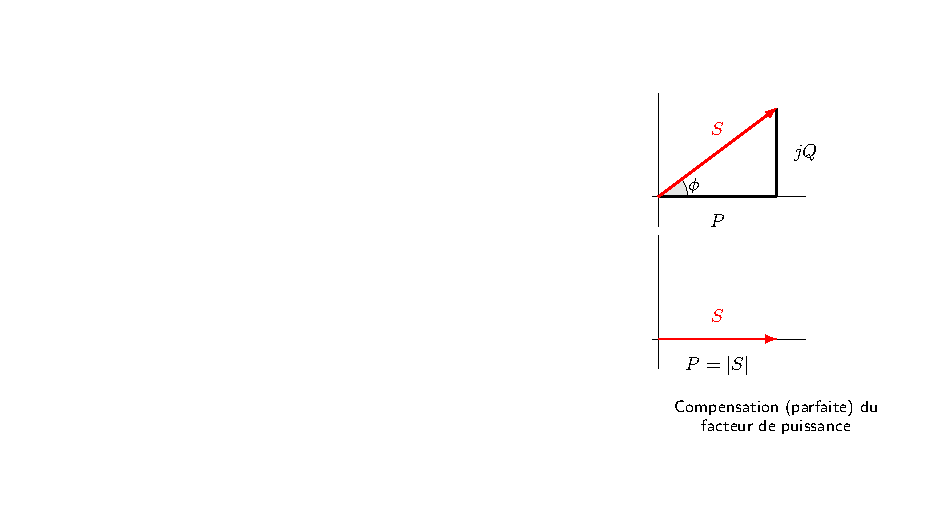
\includegraphics[width=\textwidth]{compensation_cosphi.pdf}
			\end{column}
		\end{columns}
	\end{frame}
	
	\begin{frame}[allowframebreaks]{Revenons à notre exemple : facteur de puissance}
	
	\begin{itemize}
		\item Dans le cas où L=1mH, $ \cos \phi = {0,999}$ 
		\item Dans le cas où L=100mH, $ \cos \phi = {0,302}$.
	\end{itemize}
	
	\alert{Comment rendre le facteur de puissance proche de 1 dans le deuxième cas?}

	Supposons que l'objectif est de relever le facteur de puissance à $\cos \phi' = 0,9$ en installant un condensateur de capacité $C$ en parallèle de l'ensemble $\{R, L\}$, et qu'on souhaite que la puissance active $P$ reste inchangée ($P \approx 487 \, \text{W}$). 
	
	Pour un nouveau $\cos \phi' = 0,9$, l'angle de déphasage devient :
	\[ \phi' = \arccos(0,9) \approx 25,84^\circ \]

	La nouvelle puissance réactive totale $Q_{tot}$ souhaitée est :
	\[ Q_{tot} = P \cdot \tan(\phi') = 487 \cdot \tan(25,84^\circ) \approx 235,8 \, \text{var} \]

	Calcul de la capacité $C$ : 
	le condensateur doit fournir la différence de puissance réactive entre l'état initial ($Q = 1529 \, \text{var}$) et l'état final ($Q_{tot} = 235,8 \, \text{var}$) :
	\[ Q_C = Q_{tot} - Q = 235,8 - 1529 \approx -1293,2 \, \text{var} \]

	La puissance réactive d'un condensateur est donnée par $Q_C = -\omega C V_{eff}^2$. On en déduit $C$ :
	\[ C = \frac{-Q_C}{\omega V_{eff}^2} = \frac{1293,2}{314,16 \cdot 230^2} \approx 77,8 \, \mu\text{F} \]

	Impact sur le courant : 
	grâce à cette compensation, le nouveau courant efficace appelé à la source est 
	\[ I'_{eff} = \frac{P}{V_{eff} \cdot \cos \phi'} = \frac{487}{230 \cdot 0,9} \approx 2,35 \, \text{A} \]

	\textbf{Conclusion :} En ajoutant ce condensateur, on divise le courant de ligne par près de 3 (passant de $6,98 \, \text{A}$ à $2,35 \, \text{A}$), tout en fournissant la même puissance active à la charge. Cela réduit considérablement les pertes par effet Joule dans les câbles d'alimentation.

	\alert{Question : où devrait on placer le condensateur si l'on souhaitait que la résistance consomme environ 5285 W, et quelle devrait-être la valeur de $C$?}

	\end{frame}

	%-----------------------------------------------------------------------------------
	
	\begin{frame}[allowframebreaks]{Expression de $P$ et $Q$ à partir de l'impédance (admittance) du	dipôle}

		
		Impédance $Z=R + j X$ : 
		\[S=\bar{U}\,\bar{I}^*=Z\bar{ I}\bar{I}^*=ZI^2= R\, I^2+jX\,I^2\]
		
		\begin{block}{En fonction du courant}
		\[P=R\, I^2\qquad Q= X\,I^2\]
		\end{block}		
		Admittance $Y = G + j B$ : 
		\[S=\bar{U}\,\bar{I}^*=Y^*\bar{U}\bar{U}^*=Y^*U^2= G\, U^2-jB\,U^2\]
		\begin{block}{En fonction de la tension}
			\[P=G\, U^2\qquad Q= -B\,U^2\]
		\end{block}		
				

	\end{frame}
	


	%-----------------------------------------------------------------------------------
	
	\begin{frame}[allowframebreaks]{Conservation de la puissance complexe}
		
		{\em Dans un circuit linéaire et invariant alimenté par des sources indépendantes sinusoïdales
			fonctionnant toutes à la même fréquence, la somme des puissances
			complexes fournies par les sources est égale à la somme des
			puissances complexes consommées par les éléments des autres branches
			du circuit.}
		
		\begin{columns}
			\begin{column}{0.38\linewidth}			
			\begin{center}
			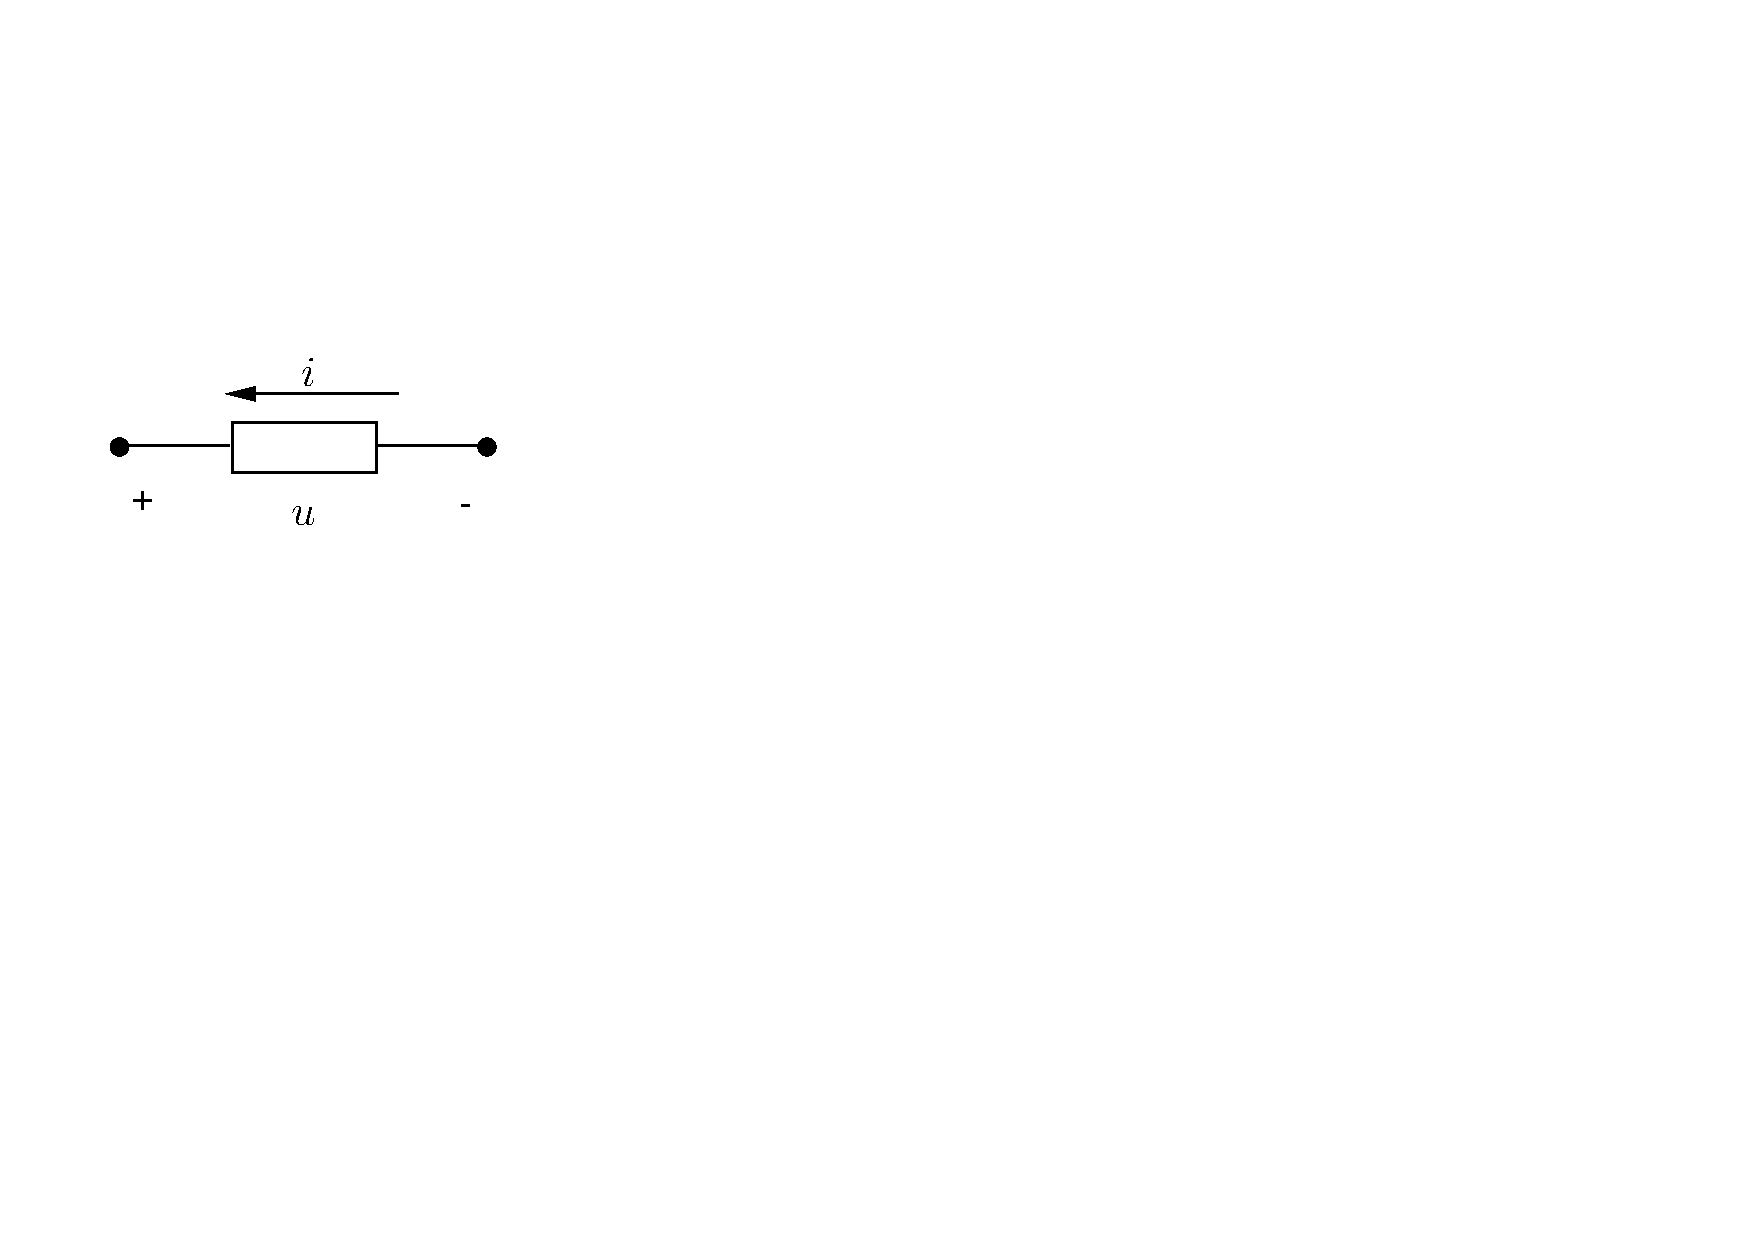
\includegraphics[width=0.7\linewidth]{conservation_S}
			\end{center}
			\end{column}
			\begin{column}{0.6\linewidth}
				Dans chaque branche,  $u_i$ et $i_i$ sont choisis dans le même sens
			\end{column}
		\end{columns}
		\begin{itemize}
			\item ${\bf i}_B$ obéit à la PLK $\rightarrow \bar{\bf I}_B^*$ obéit aussi
			à la PLK
			\item ${\bf u}_B$ obéit à la SLK $\rightarrow \bar{\bf U}_B$ obéit aussi
			à la SLK
			\item $\bar{\bf I}_B^*$,  $\bar{\bf U}_B$ satisfont le théorème de
			Tellegen et 
			\[\bar{\bf I}_B^*\bar{\bf U}_B=0\]
		\end{itemize}
		\[\bar{\bf I}_B^*\bar{\bf U}_B=\sum_{i=1}^b\bar{U}_i\bar{I}_i^* = S
		\quad \text{est la puissance complexe totale fournie au circuit.}\]
	\end{frame}
	
	%-----------------------------------------------------------------------------------

%	\begin{frame}{Propriétés des impédances de dipôles RLC passifs}
%		On suppose :
%		\begin{itemize}
%			\item circuit constitué d'éléments RLC passifs ($R>0$, $L>0$, $C>0$)
%			\item un seul élément par branche 
%		\end{itemize}
%		\begin{center}
%			%TODO \input{propimpch10.pstex_t}
%			
%			\[\text{Re}[Z(j\omega)]\geq 0 \qquad -90^{\circ}\leq
%			\text{arg}[Z(j\omega)]\leq 90^{\circ}\]
%		\end{center}
%	\end{frame}
	
	%-----------------------------------------------------------------------------------
	
%	\begin{frame}{Impédance d'un dipôle}
%		Conservation de la puissance complexe 
%		\[\bar{U}_1\bar{I}_1^*=-\sum_{i=2}^b\bar{U}_i\bar{I}_i^*\]
%		L'impédance du dipôle est donnée par
%		{\small \[Z(j\omega)=\frac{\bar{U}_1}{\bar{I}_1}\]}
%		et pour chaque branche
%		{\small \[Z_i(j\omega)=-\frac{\bar{U}_i}{\bar{I}_i}=
%			\begin{cases}
%			R_i & \text{si la branche est résistive}\\
%			j\omega L_i & \text{si la branche est inductive}\\
%			\frac{-j}{\omega C_i} & \text{si la branche est capacitive} 
%			\end{cases}\]}
%		
%		{\small \[Z(j\omega)I_1^2=\sum_{R_i}R_i I_i^2 + \sum_{L_i}j\omega
%			L_i I_i^2+\sum_{C_i}\frac{-j}{\omega C_i}I_i^2\]}
%		
%	\end{frame}
	
	%-----------------------------------------------------------------------------------
	
%	\begin{frame}{Remarques}
%		 \[\text{Re}[Z(j\omega)]=\sum_{R_i}R_i\frac{I_i^2}{I_1^2} \qquad
%			\text{Im}[Z(j\omega)]=\sum_{L_i}\omega L_i\frac{I_i^2}{I_1^2}
%			-\sum_{C_i}\frac{1}{\omega C_i}\frac{I_i^2}{I_1^2}\]
%			\begin{itemize}
%				\item on a toujours $\text{Re}[Z(j\omega)] \geq 0$
%				\item circuit purement résistif : $\text{Re}[Z(j\omega)] > 0$, 
%				$\text{Im}[Z(j\omega)]=0$, $\text{arg}[Z(j\omega)]=0$ \\
%				impédance purement résistive
%				\item circuit purement inductif : $\text{Re}[Z(j\omega)] =0$, 
%				$\text{Im}[Z(j\omega)] >0$, $\text{arg}[Z(j\omega)]=90^{\circ}$
%				impédance purement réactive, selfique
%				\item circuit purement capacitif : $\text{Re}[Z(j\omega)] =0$, 
%				$\text{Im}[Z(j\omega)] < 0$, $\text{arg}[Z(j\omega)]=-90^{\circ}$\\
%				impédance purement réactive, capacitive
%				\item circuit RL : $\text{Re}[Z(j\omega)] >0$, 
%				$\text{Im}[Z(j\omega)] > 0$, $0 < \text{arg}[Z(j\omega)]
%				<90^{\circ}$
%				\item circuit RC : $\text{Re}[Z(j\omega)] >0$, 
%				$\text{Im}[Z(j\omega)] < 0$, $-90^{\circ} < \text{arg}[Z(j\omega)]
%				<0$
%				\item circuit LC :
%				$\text{Re}[Z(j\omega)] = 0$, 
%				$\text{arg}[Z(j\omega)]=\pm 90^{\circ}$\\
%				impédance purement réactive, selfique ou capacitive selon que
%				l'énergie moyenne magnétique est supérieure ou inférieure à l'énergie moyenne 
%				électrostatique 
%				\item cas général du circuit RLC : $\text{Re}[Z(j\omega)] > 0$, 
%				$-90^{\circ}< \text{arg}[Z(j\omega)] <  90^{\circ}$
%			\end{itemize}
%		\end{frame}
%		
		%-----------------------------------------------------------------------------------
		
		\begin{frame}{Synthèse}
			\begin{center}
				{\small \begin{tabular}{lrrrr}
						\hline
						Dipôle & arg$[Z]$ & $\cos \Phi$ & $P$ & $Q$\\ \hline
						R & 0 & 1 & $P>0$ & $Q=0$\\
						L & $90^{\circ}$ & 0 & $P=0$ & $Q=\omega L I^2 > 0$\\
						C & $-90^{\circ}$ & 0 & $P=0$ & $Q=-\omega C U^2 <0$\\
						LC & $\pm 90^{\circ}$ & 0 & $P=0$ & $Q > < 0$\\
						RL & $0< \Phi < 90^{\circ}$ & $0 < \cos \Phi < 1$ & $P>0$ & $Q>0$\\
						RC & $-90^{\circ}< \Phi < 0$ & $0 < \cos \Phi < 1$& $P>0$  & $Q<0$
						\\ \hline
				\end{tabular}}
			\end{center}
			
			
			{\small $P$ et $Q$ sont les puissances consommées par le dipôle.}
		\end{frame}
			
	%-----------------------------------------------------------------------------------
\section{Circuits magnétiquement couplés}

\subsection{Inductances couplées}
\begin{frame}{Inductances couplées}
	
	Eléments linéaires et invariants.
	
	\begin{columns}
		\begin{column}{0.5\linewidth}
			\begin{center}
				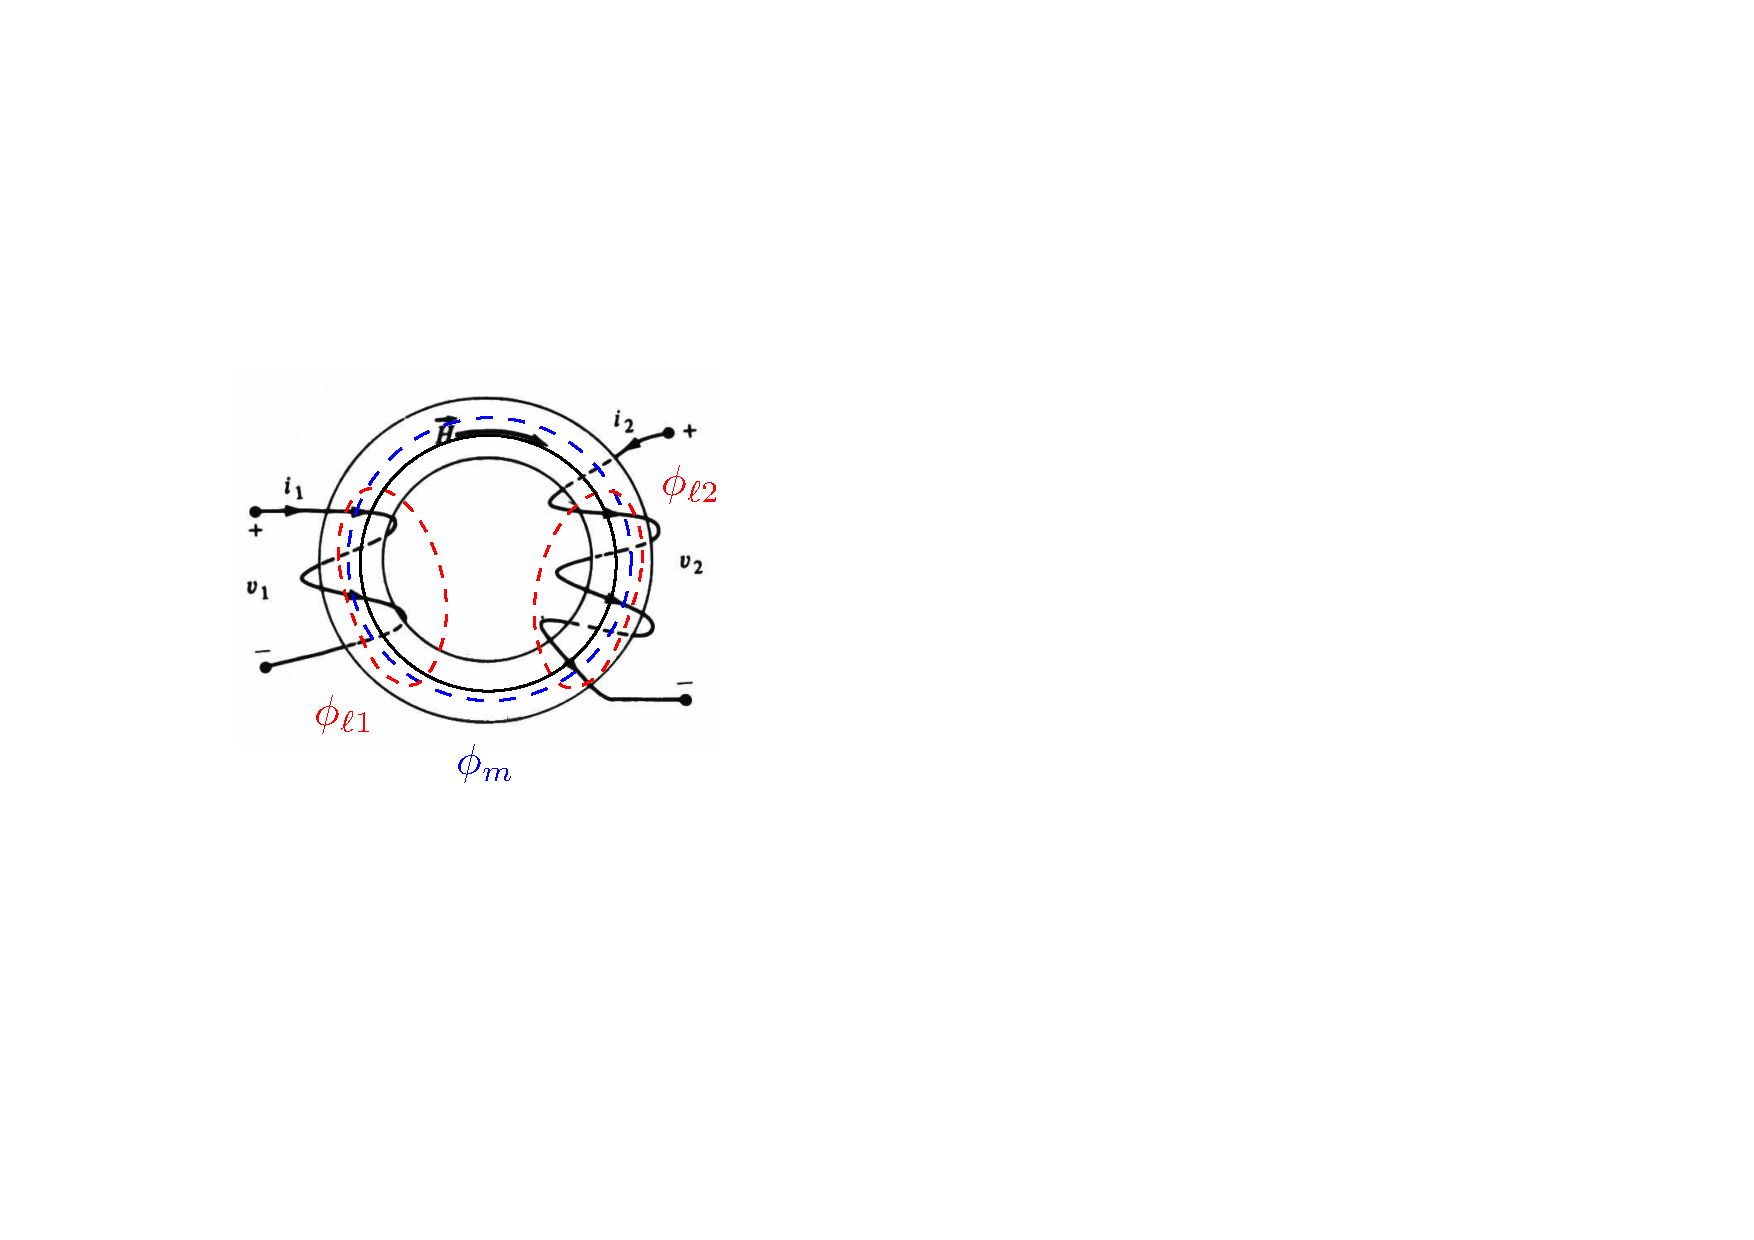
\includegraphics[width=0.7\linewidth]{CMC_principe}
			\end{center}
		\end{column}
		\begin{column}{0.5\linewidth}
			Deux circuits magnétiquement couplés.
			
			Flux produit par $i_1$ embrasse la bobine 2 et inversement.
			
			$\rightarrow$ courant variable $i_1$ induit une f.e.m aux bornes de la bobine 2.
		\end{column}
	\end{columns}
	
	$N_1$ : nombre de tours de la bobine 1\\
	$N_2$ : nombre de tours de la bobine 2
	
\end{frame}

%---------------------------------------------------------------------

\begin{frame}{Relations entre courants et tensions}
	
	Si $i_1$ agit seul et que le circuit 2 est ouvert, 
	le flux généré par $i_1$ se décompose en 
	\[\phi_1^{(1)}=\phi_{l1}+\phi_m^{(1)}\]
	$\phi_{l1}$ : partie du flux qui traverse uniquement la bobine 1 (flux de fuite)\\
	$\phi_m^{(1)}$ : partie du flux qui traverse à la fois la bobine 1 et la bobine 2
	
	\vfill
	Tensions induites :
	\begin{eqnarray*}
		u_1^{(1)} & = &N_1\frac{d\phi_1^{(1)}}{dt}=N_1\frac{d(\phi_{l1}+\phi_m^{(1)})}{dt}=L_1\frac{di_1}{dt}\\
		u_2^{(1)} & = & N_2\frac{d\phi_m^{(1)}}{dt}=L_{21}\frac{di_1}{dt}
	\end{eqnarray*}
	
\end{frame}

%---------------------------------------------------------------------

\begin{frame}{Relations entre courants et tensions}
	
	Si $i_2$ agit seul et que le circuit 1 est ouvert, le flux généré par $i_2$ se décompose en 
	\[\phi_2^{(2)}=\phi_{l2}+\phi_m^{(2)}\]
	
	Tensions induites :
	\begin{eqnarray*}
		u_1^{(2)} & = &N_1\frac{d\phi_m^{(2)}}{dt}=L_{12}\frac{di_2}{dt}\\
		u_2^{(2)} & = & N_2\frac{d\phi_2^{(2)}}{dt}=L_2\frac{di_2}{dt}
	\end{eqnarray*}
	
	\begin{block}{Inductance mutuelle $M$}
		
		On a $L_{12}=L_{21}=M$, l'inductance mutuelle.
		
		$M$ dépend de la géométrie du système, de la distance et de
		l'orientation relative entre les deux bobines.
	\end{block}
	
\end{frame}	
%---------------------------------------------------------------------
\begin{frame}{Relations entre courants et tensions}	
	
	Par superposition, si $i_1$ et $i_2$ agissent simultanément
	\begin{eqnarray*}
		u_1& = &L_1\frac{di_1}{dt}+M\frac{di_2}{dt}\\
		u_2& = &M\frac{di_1}{dt}+L_2\frac{di_2}{dt}
	\end{eqnarray*}
	
	\begin{block}{Modèle de deux inductances couplées}
		\begin{columns}
			\begin{column}{0.5\linewidth}
				\[\left[
				\begin{array}{c}
				u_1\\
				u_2
				\end{array}\right] = \left[
				\begin{array}{cc}
				L_1 & M \\
				M & L_2
				\end{array}\right]
				\frac{d}{dt}\left[
				\begin{array}{c}
				i_1\\i_2
				\end{array}\right]\]
			\end{column}
			\begin{column}{0.5\linewidth}
				\begin{center}
					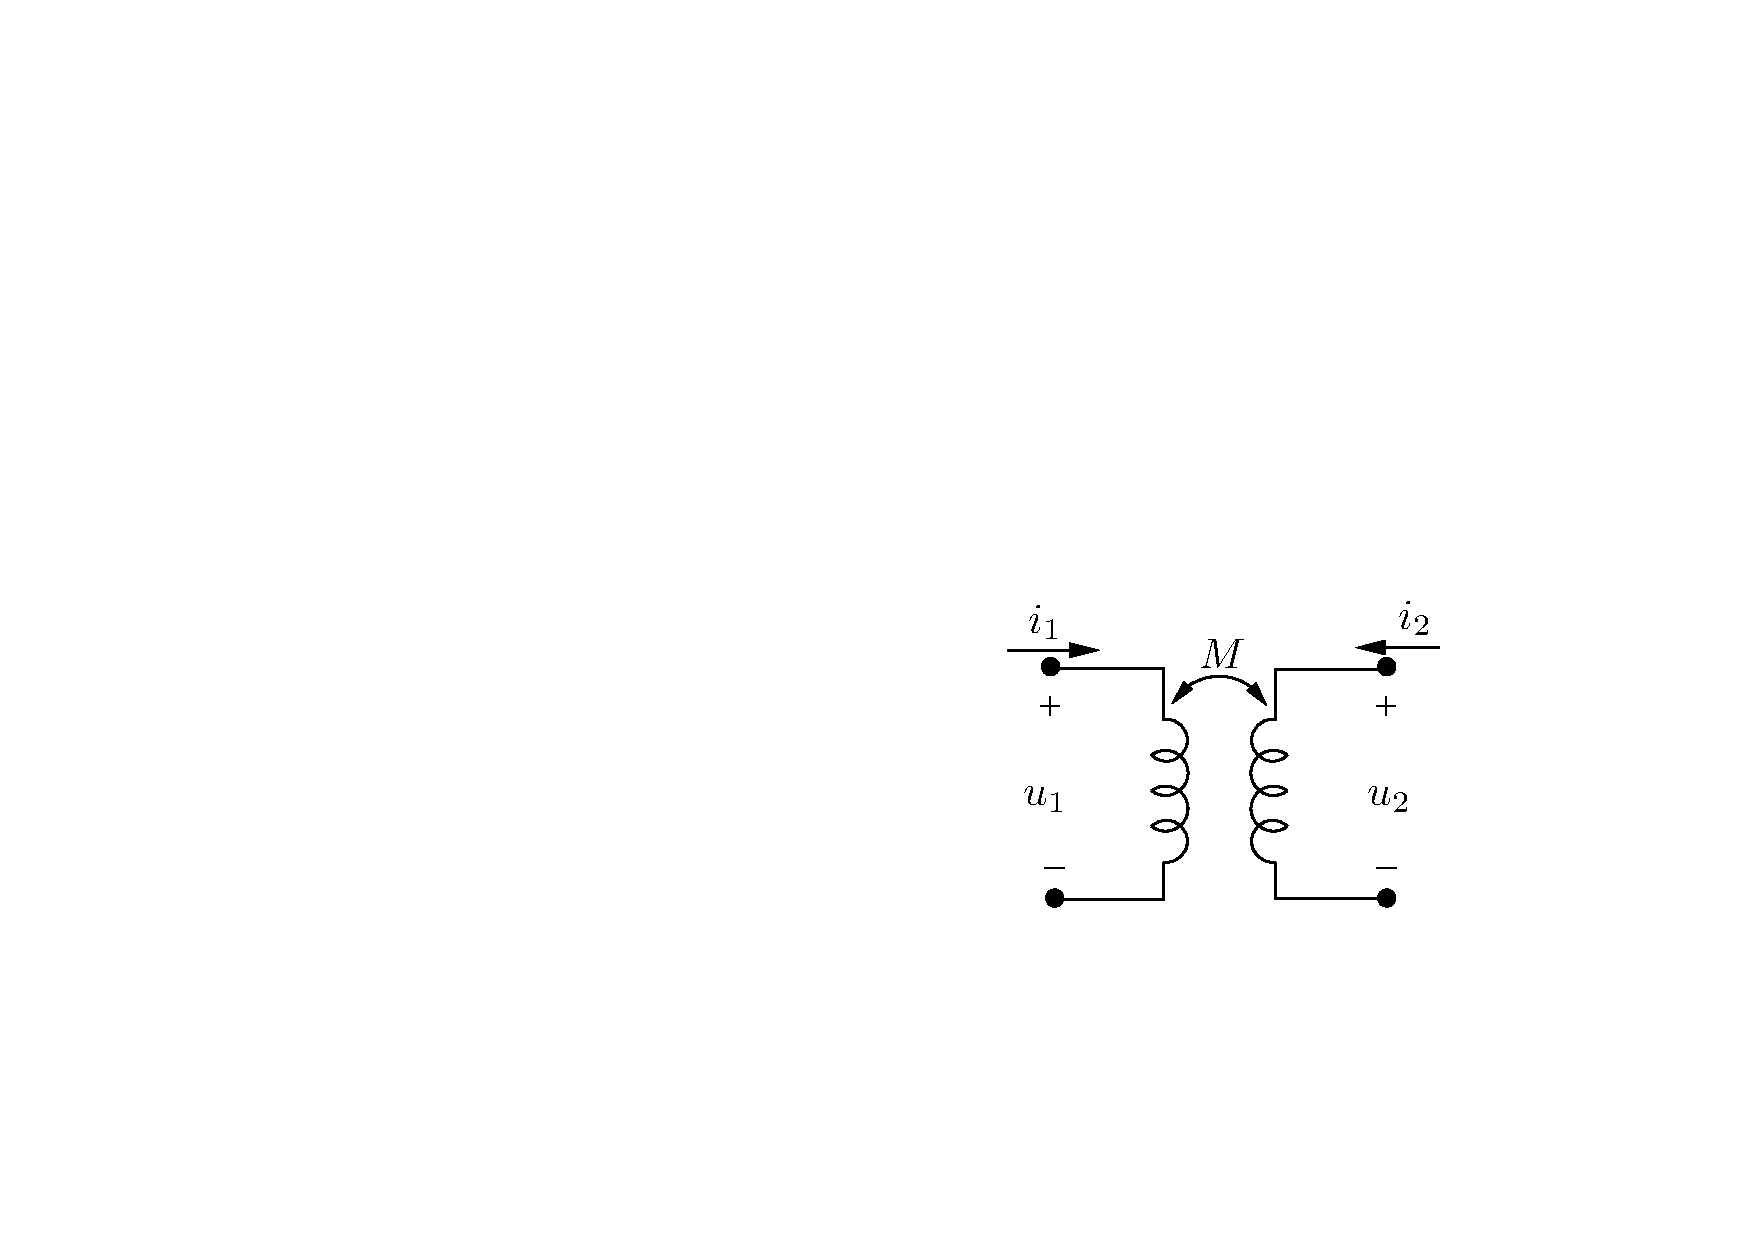
\includegraphics[width=0.6\linewidth]{CMC_schematic}
				\end{center}
			\end{column}
		\end{columns}
	\end{block}
\end{frame}

%---------------------------------------------------------------------

\begin{frame}{Signe de $M$}
	Selon l'arrangement des bobines, $M$ est positif ou négatif
	
	\begin{columns}
		\begin{column}{0.5\linewidth}
			\begin{center}
				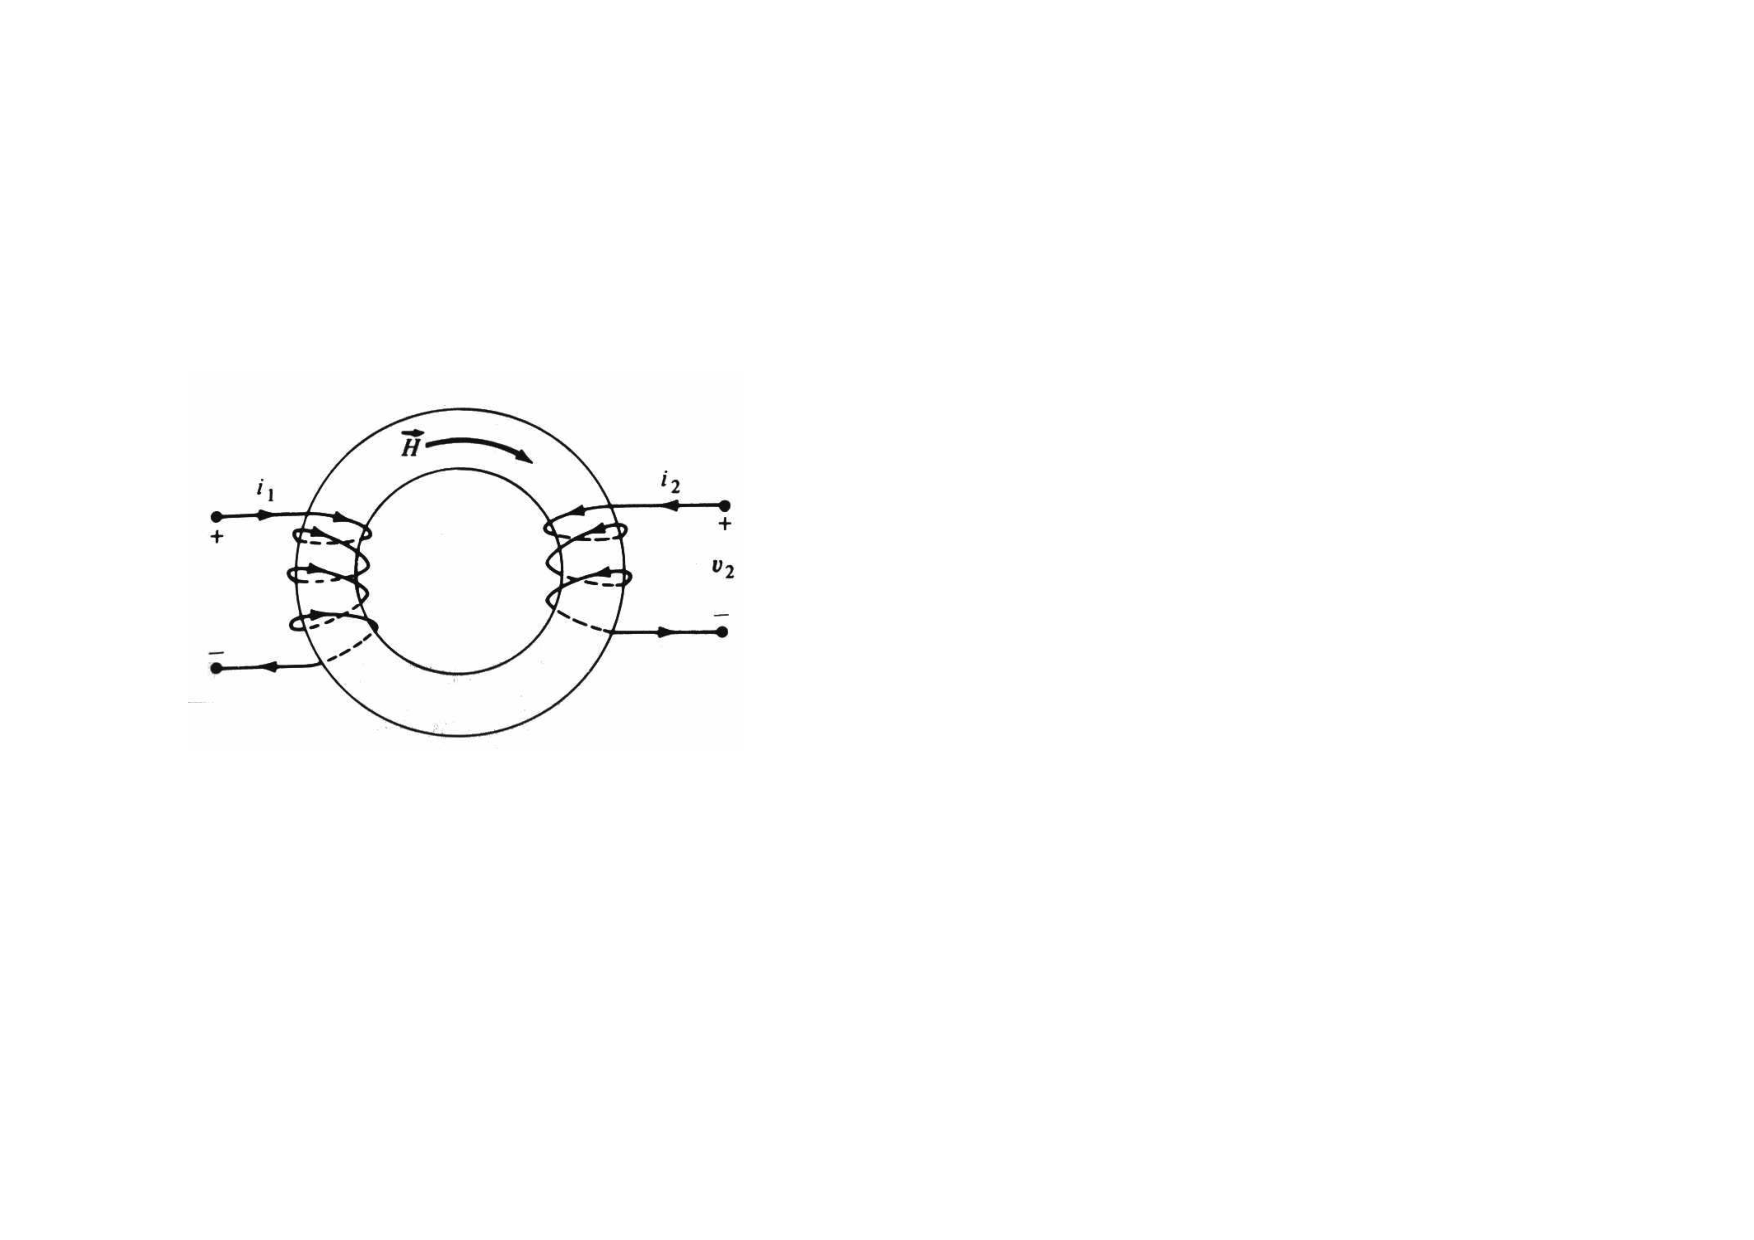
\includegraphics[width=0.6\linewidth]{CMC_cas1}\\
				$M>0$\\
				$\phi_m^{(1)}$ et $\phi_m^{(2)}$ dans le même sens\\
				ils s'ajoutent
			\end{center}
		\end{column}
		\begin{column}{0.5\linewidth}
			\begin{center}
				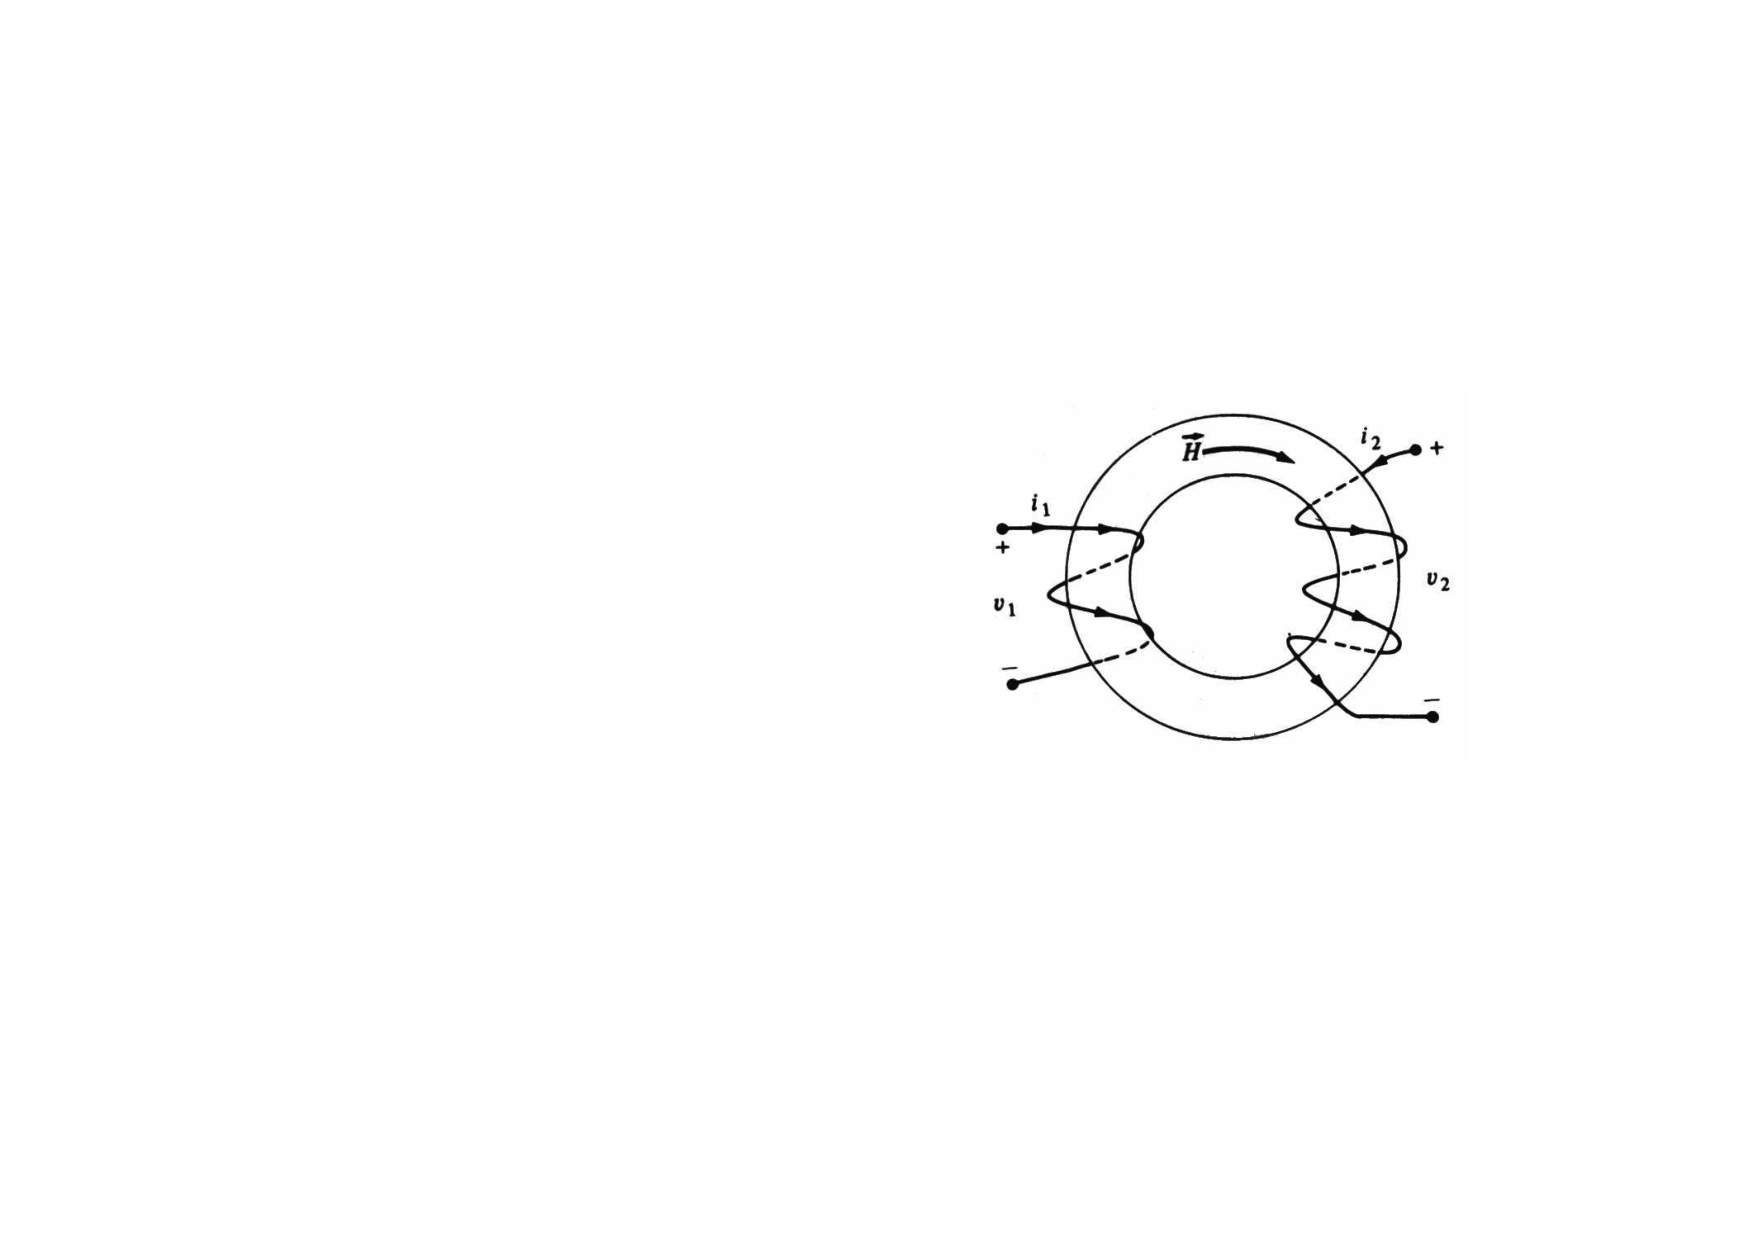
\includegraphics[width=0.6\linewidth]{CMC_cas2}\\
				$M<0$\\
				$\phi_m^{(1)}$ et $\phi_m^{(2)}$ en sens opposés\\
				ils se soustraient
			\end{center}
		\end{column}
	\end{columns}	
\end{frame}

%---------------------------------------------------------------------

\begin{frame}{Indication du signe de $M$}
	Sur le schéma, on repère le signe de $M$ par des points :
	
	$M>0$ si $i_1$ et $i_2$ entrent ou sortent tous les deux par la borne
	dotée d'un point.
	\begin{center}
		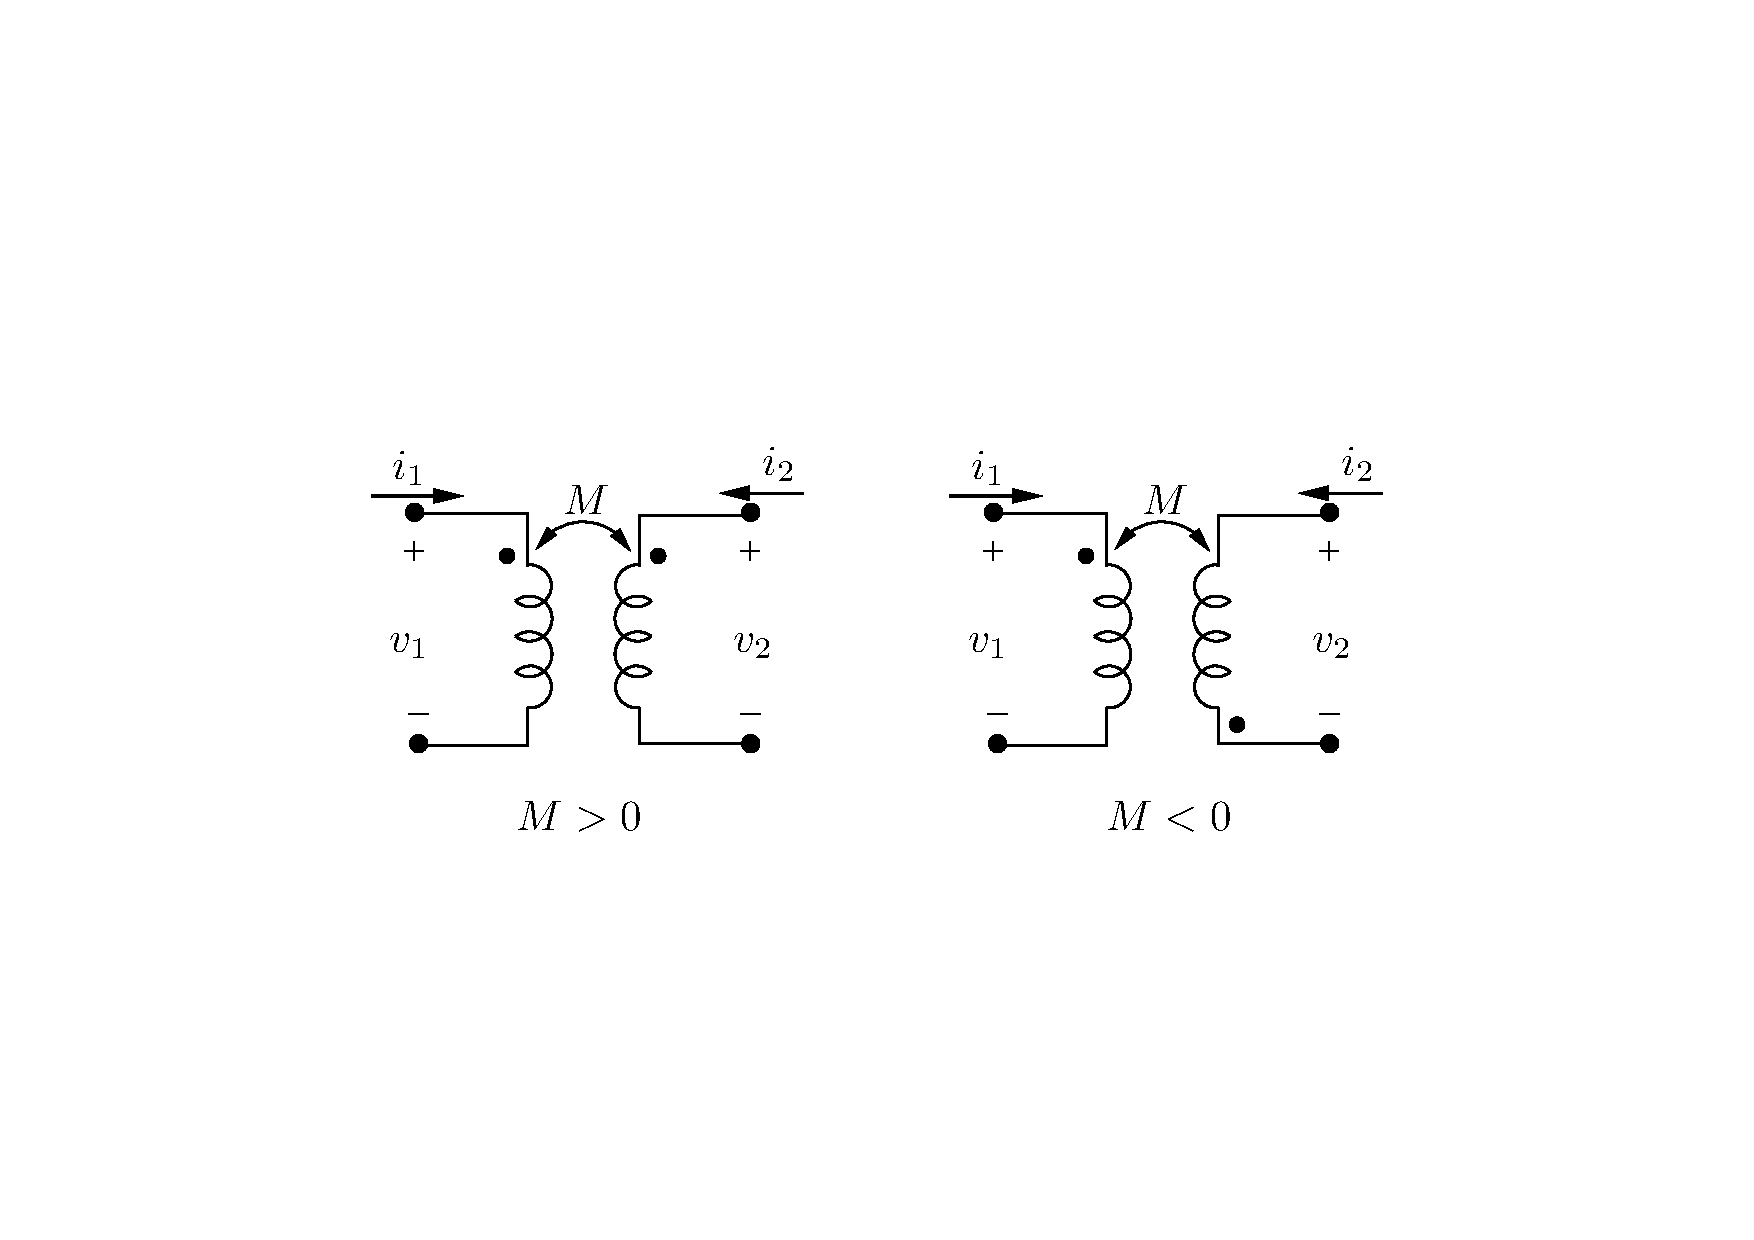
\includegraphics[width=0.9\linewidth]{CMC_symbols}
	\end{center}
\end{frame}

%---------------------------------------------------------------------

\begin{frame}{Coefficient de couplage $k$}
	
	\begin{block}{Coefficient de couplage}
		\[M=k\sqrt{L_1L_2}\]
		\[-1\leq k \leq 1\]
	\end{block}
	
	Cas extrêmes : 
	\begin{itemize}
		\item $k=0$ : aucun couplage entre les deux bobines; le flux créé par
		chaque bobine ne traverse que cette bobine.
		\item $|k|=1$ : couplage parfait; tout le flux créé par chaque bobine
		traverse l'autre bobine.
	\end{itemize}
\end{frame}

%---------------------------------------------------------------------

\subsection{Le transformateur et le transformateur idéal}
\begin{frame}{Le transformateur}
	
	Deux enroulements  magnétiquement  couplés = une paire d'inductances couplées.
	\vfill
	Utile pour
	\begin{itemize}
		\item adapter le niveau de tension : transport et distribution de
		l'énergie électrique
		\item adapter l'impédance d'un circuit à une impédance de charge :
		circuits électroniques, télécom
		\item réaliser des mesures de courant et de tension : voir cours de
		Mesures Electriques
	\end{itemize}
	
	\vfill
	\begin{columns}
		\begin{column}{0.5\linewidth}
			Modèle ``réaliste'' : une paire d'inductances couplées + une
			résistance pour chaque enroulement (pertes).
		\end{column}
		\begin{column}{0.5\linewidth}
			\begin{center}
				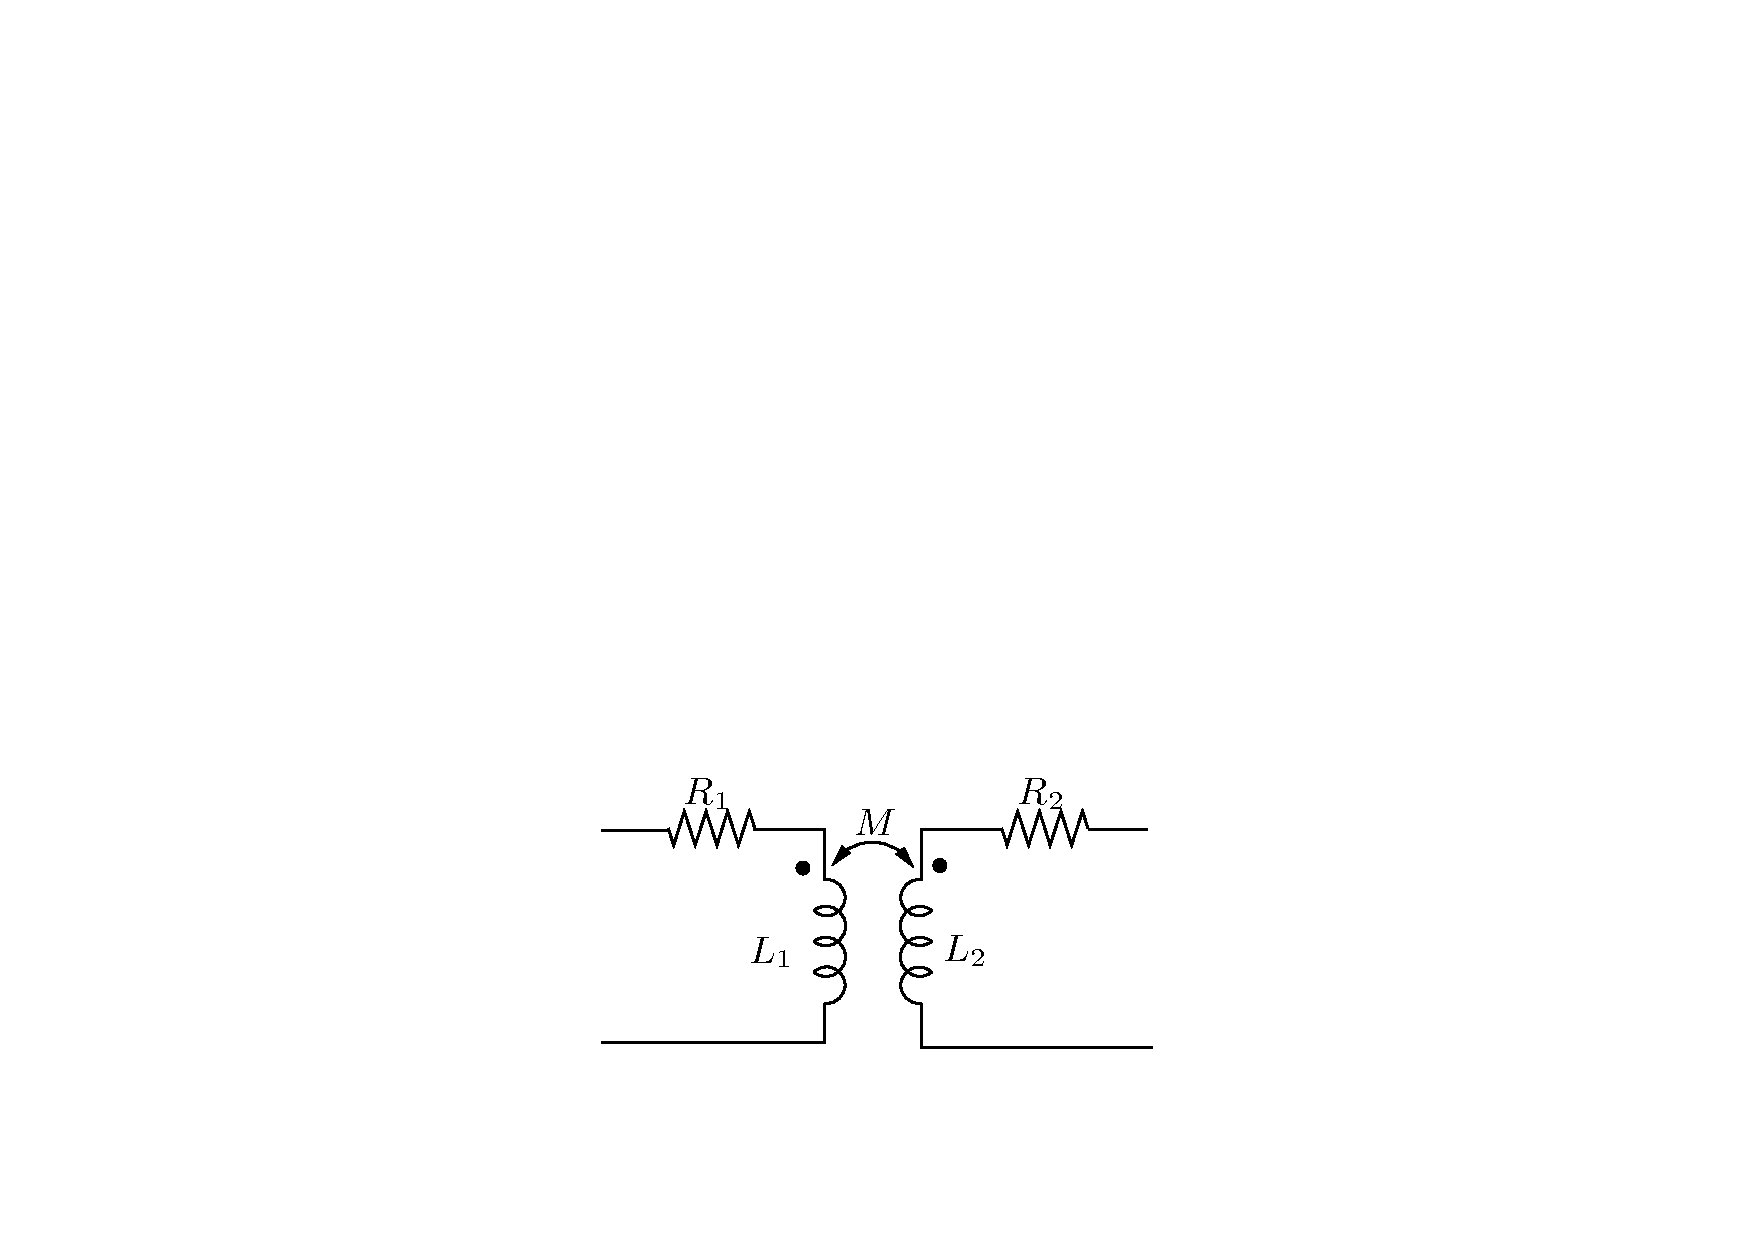
\includegraphics[width=0.8\linewidth]{transfo}
			\end{center}
		\end{column}
	\end{columns}
\end{frame}
%---------------------------------------------------------------------

\begin{frame}{Le transformateur idéal}
	
	Idéalisations :
	\begin{itemize}
		\item $R_1=R_2=0$
		\item couplage parfait : $k=1$, pas de flux de fuite
		\item matériau ferromagnétique idéal : $\mu=\infty \rightarrow
		L_1\rightarrow \infty$, $L_2\rightarrow \infty$, $M\rightarrow \infty$
	\end{itemize}
	
	On peut écrire :
	{\[\left[
		\begin{array}{c}
		u_1\\
		\frac{di_1}{dt}
		\end{array}\right] = \left[
		\begin{array}{cc}
		\frac{L_1}{M} & M-\frac{L_1L_2}{M} \\
		\frac{1}{M} & -\frac{L_2}{M}
		\end{array}\right]
		\left[
		\begin{array}{c}
		u_2\\ \frac{di_2}{dt}
		\end{array}\right]\]}
	Tenant compte des idéalisations
	{\[\left[
		\begin{array}{c}
		u_1\\
		\frac{di_1}{dt}
		\end{array}\right] = \left[
		\begin{array}{cc}
		\sqrt{\frac{L_1}{L_2}}  & 0\\
		0 & -\sqrt{\frac{L_2}{L_1}}
		\end{array}\right]
		\left[
		\begin{array}{c}
		u_2\\ \frac{di_2}{dt}
		\end{array}\right]
		\]}
\end{frame}

%---------------------------------------------------------------------

\begin{frame}{Modèle du transformateur idéal}
	
	On pose 
	\[n=\frac{L_2}{M}=\frac{M}{L_1}=\sqrt{\frac{L_2}{L_1}}=\frac{N_2}{N_1}\]
	
	et on obtient les relations qui caractérisent l'élément ``transformateur idéal''.
	
	\begin{block}{Modèle du transformateur idéal}
		\begin{columns}
			\begin{column}{0.5\linewidth}
				\begin{eqnarray*}
					u_2& = &nu_1\\
					i_1 & = & -ni_2
				\end{eqnarray*}
			\end{column}
			\begin{column}{0.5\linewidth}
				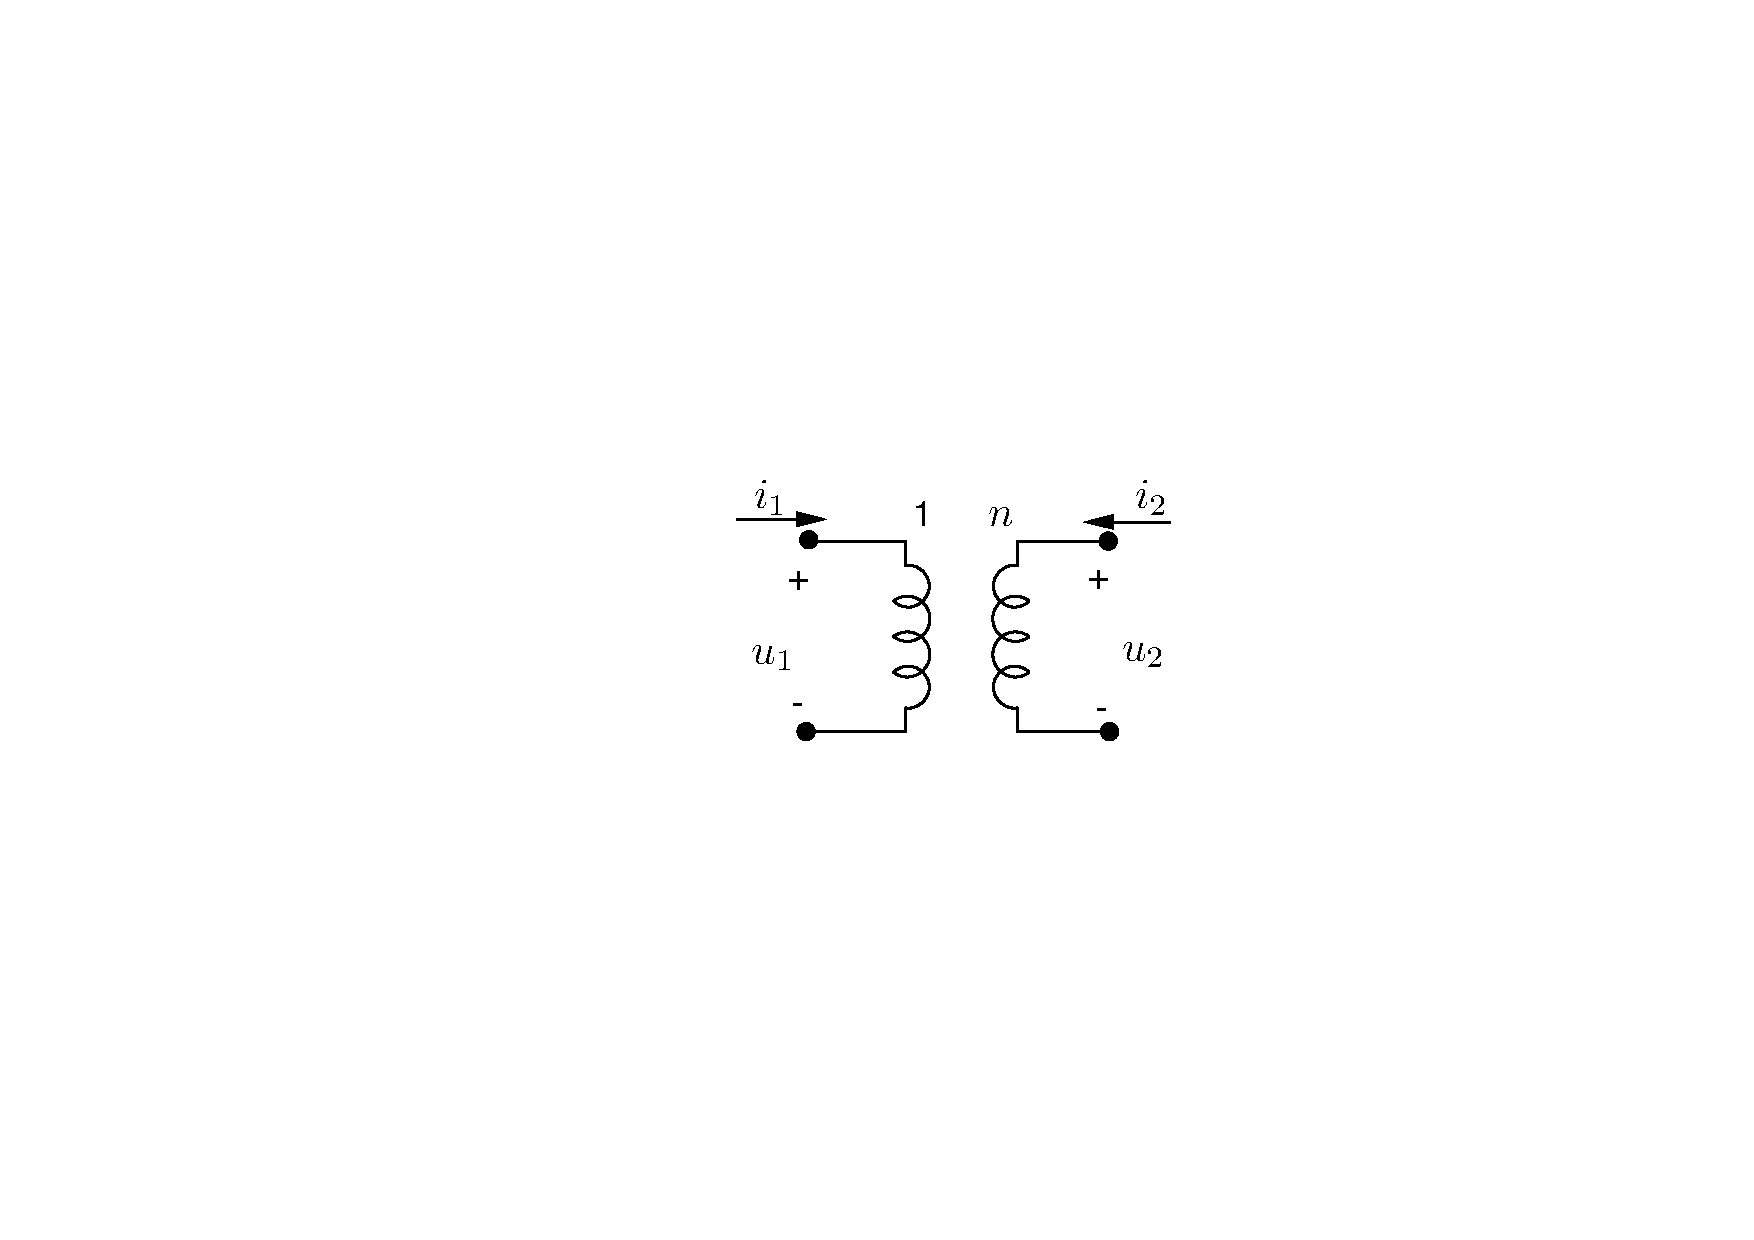
\includegraphics[width=0.7\linewidth]{transfo_UetI}
			\end{column}
		\end{columns}
	\end{block}	
	
	Le transformateur idéal est un quadripôle.
	
	$n$ est le rapport de transformation.
\end{frame}

\subsection{Synthèse : classification énergétique des élémens}
\begin{frame}{Synthèse : classification énergétique des éléments}
Soit $w(t)$ l'énergie emmagasinée dans un élément d'un circuit à un instant $t$, et $p(t)$ la puissance instantanée consommée par cet élément. On peut catégoriser les éléments comme ceci : 
	\begin{center}
		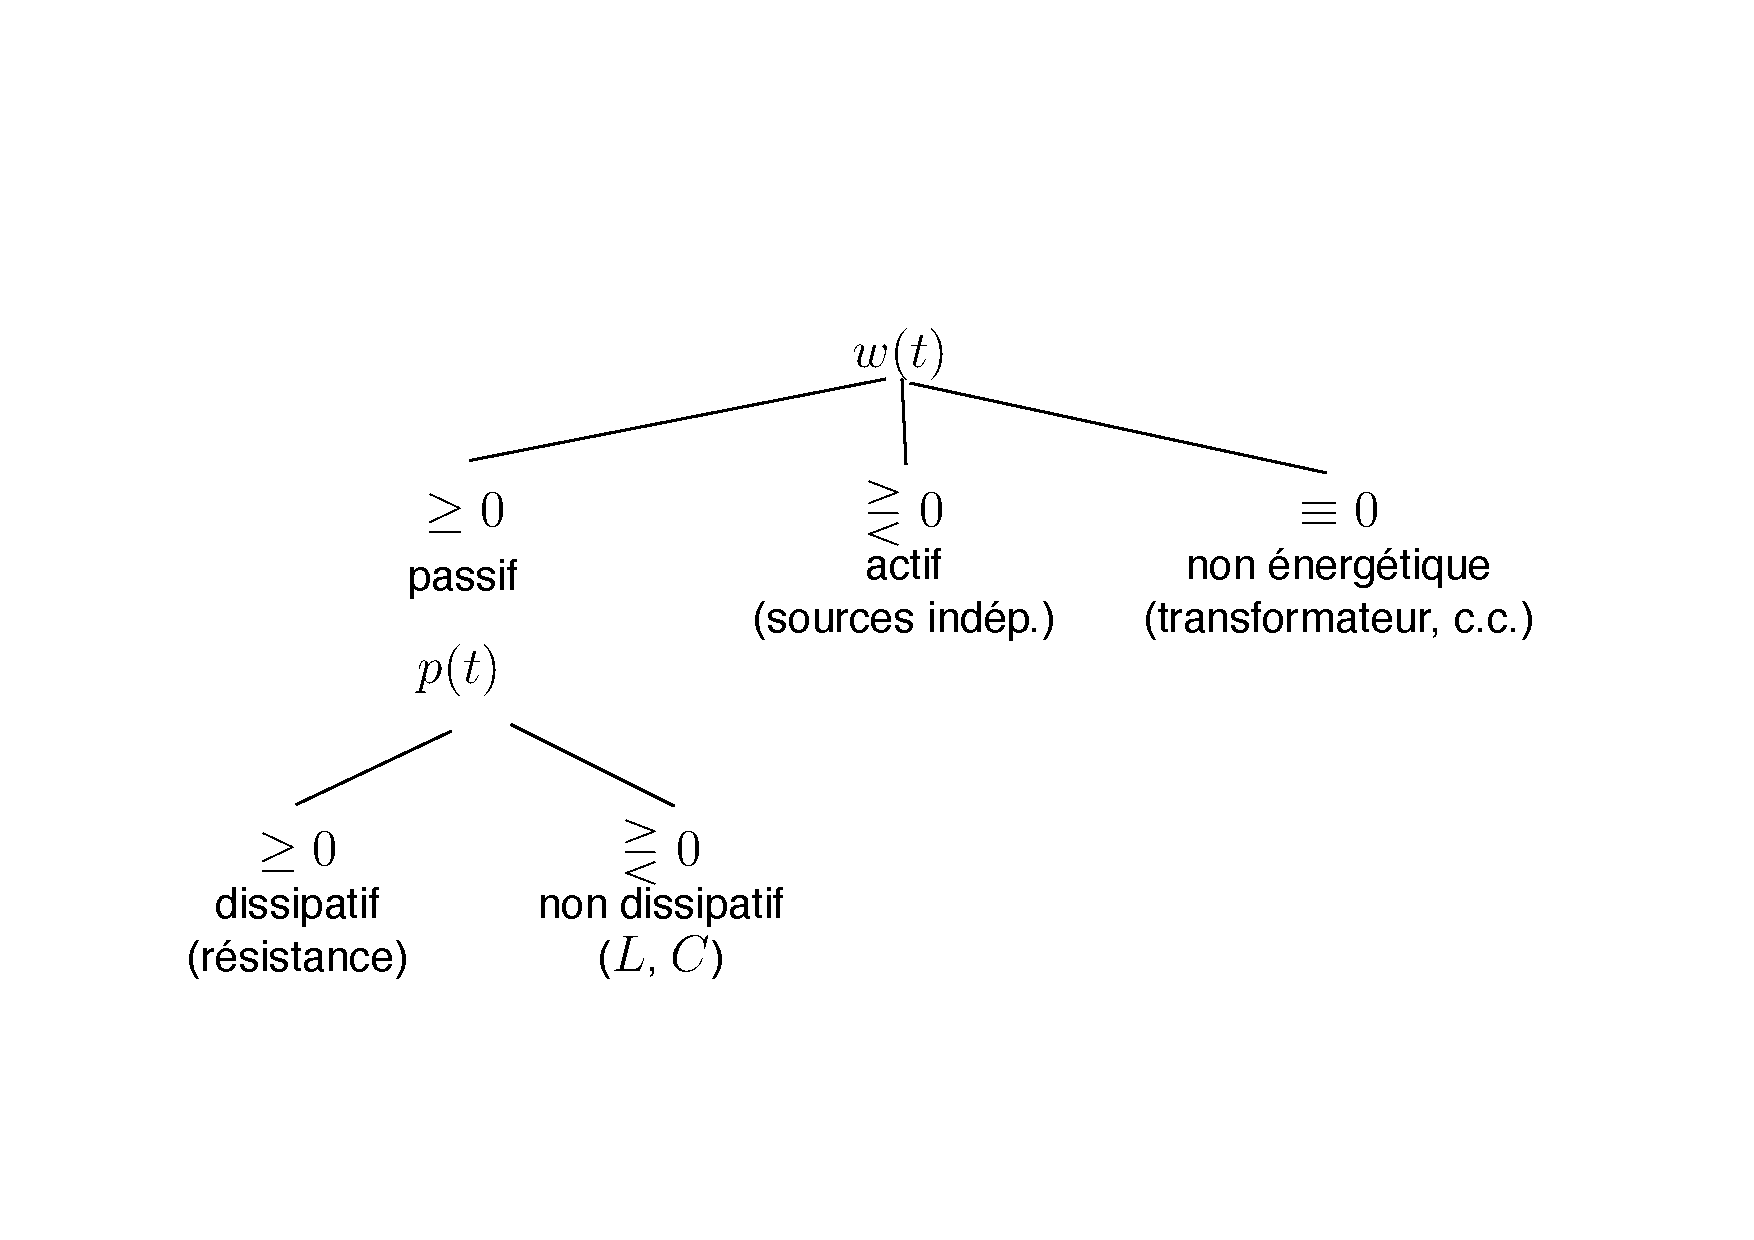
\includegraphics[width=0.6\linewidth]{classification}
	\end{center}
\end{frame}




\section{Circuits triphasés équilibrés}
	
\begin{frame}{Introduction}
	Le transport et la distribution de l'énergie électrique sont réalisés au moyen
	de systèmes triphasés fonctionnant en régime sinusoïdal, à l'exception
	de quelques liaisons haute tension à courant continu.
	
	\vfill
	Le transport utilise des systèmes à THT (très haute tension, 700 à 150 kV).
	
	\vfill
	La distribution utilise des systèmes BT (basse tension, qq kV à qq
	100taines V).
	
	\vfill
	Pourquoi ?
	\begin{itemize}
		\item THT permet de réduire les pertes par effet Joule dans les conducteurs
		\item régime sinusoïdal permet l'utilisation de transformateurs pour
		abaisser ou élever les niveaux de tension
		\item régime triphasé 
		\begin{itemize}
			\item permet la création de champs tournants (moteurs, alternateurs)
			\item économie de conducteurs pour transporter une même puissance
			\item puissance instantanée fournie à la charge triphasée constante
		\end{itemize}
	\end{itemize}
\end{frame}


\begin{frame}{Principe}
	
	Un circuit \textbf{triphasé} est constitué de trois circuits appelés {\em phases}. 
	
	\vfill
	
	Un système est \textbf{équilibré} si tous ses constituants le sont.
	
	\vfill 
	
	Eléments triphasés : 
	\begin{itemize}
		\item générateur : circuit à 3 accès qui délivre 3 f.e.m, équilibré si
		les f.e.m sont égales en amplitude et déphasées temporellement
		entre elles d'un tiers de période et si chaque phase présente une
		impédance interne identique;
		\item charge : circuit à 3 accès, équilibré si chaque phase est
		constituée d'une impédance identique;
		\item circuit de transmission : relie la charge au générateur,
		équilibré si chaque phase possède une impédance identique.
	\end{itemize}
\end{frame}


\begin{frame}{}
\begin{center}
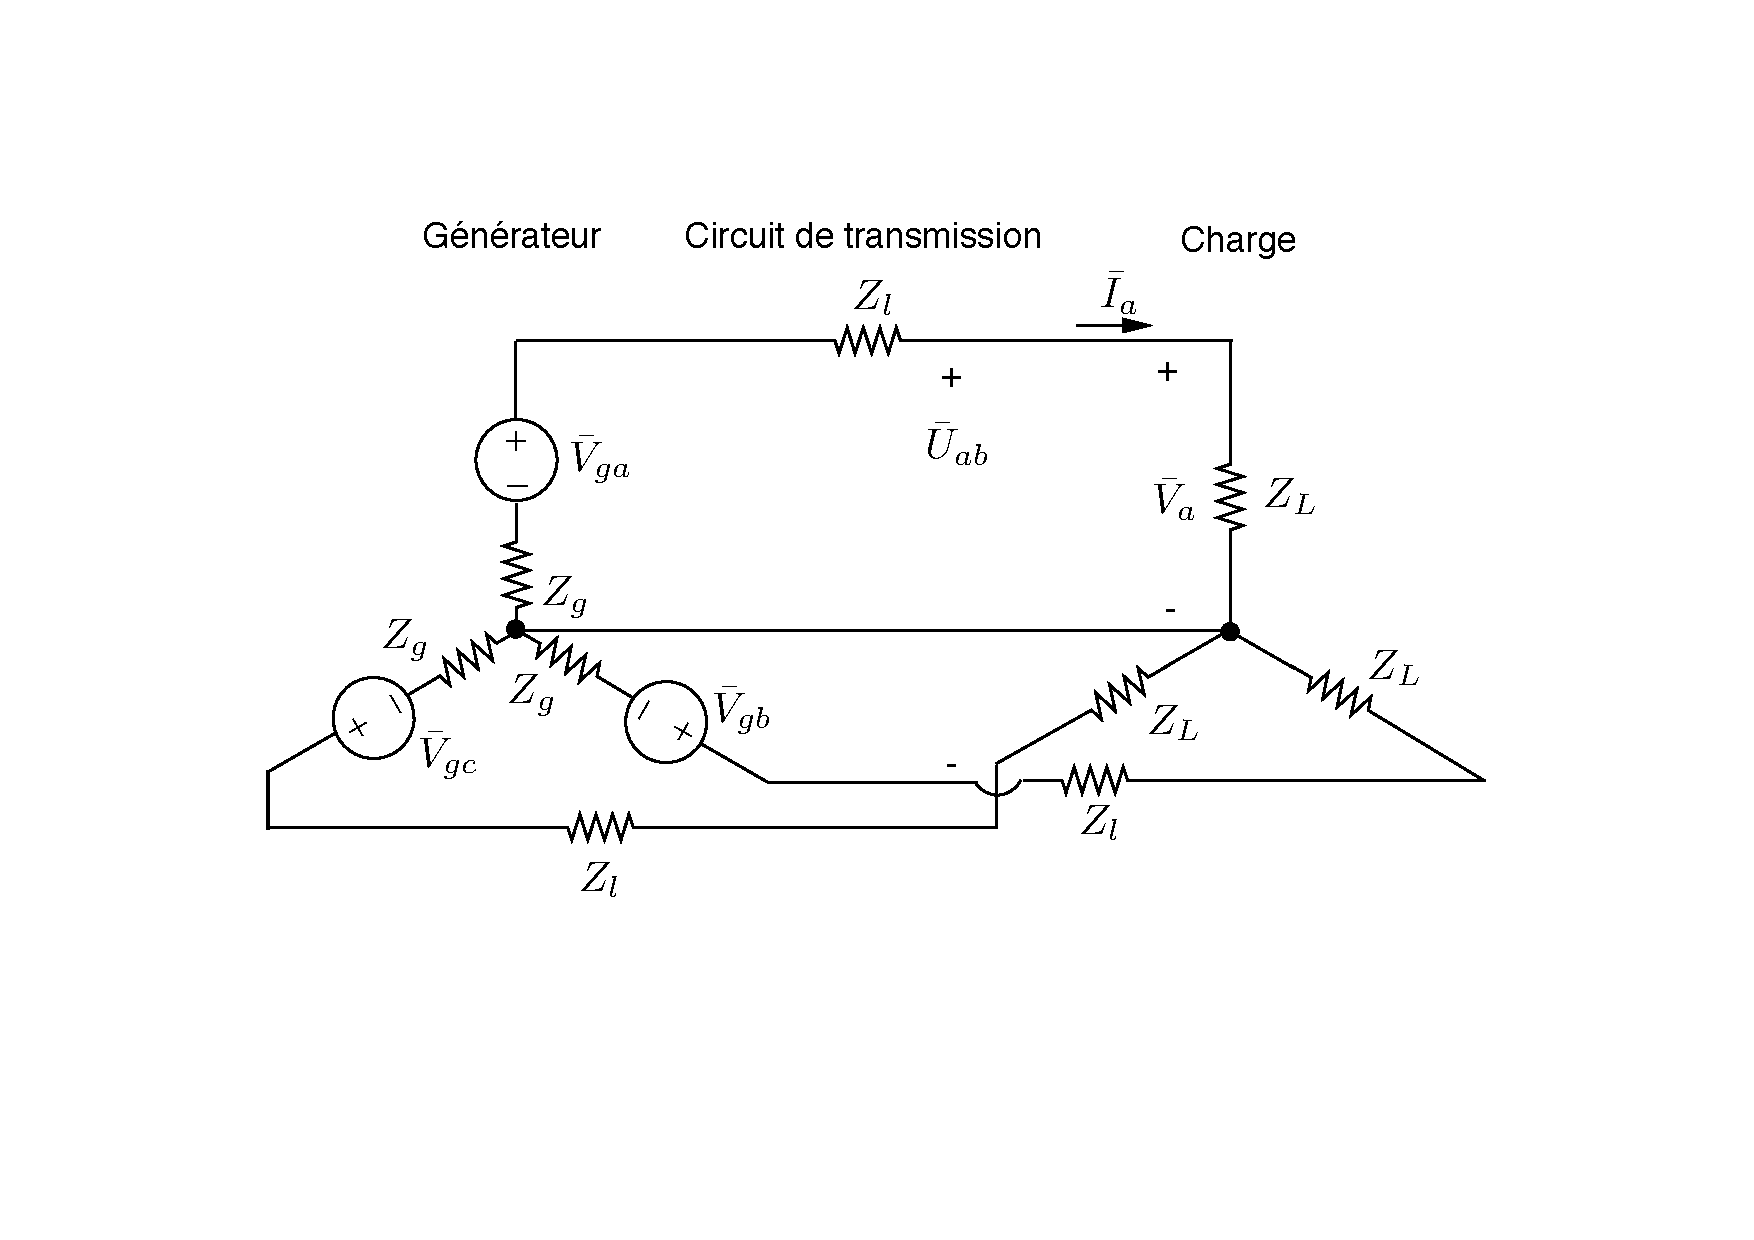
\includegraphics[width=1\linewidth]{principe_3phase}
\end{center}
\end{frame}


\begin{frame}{Générateur triphasé équilibré}
	
	\begin{columns}
		\begin{column}{0.5\linewidth}		
		\begin{center}
		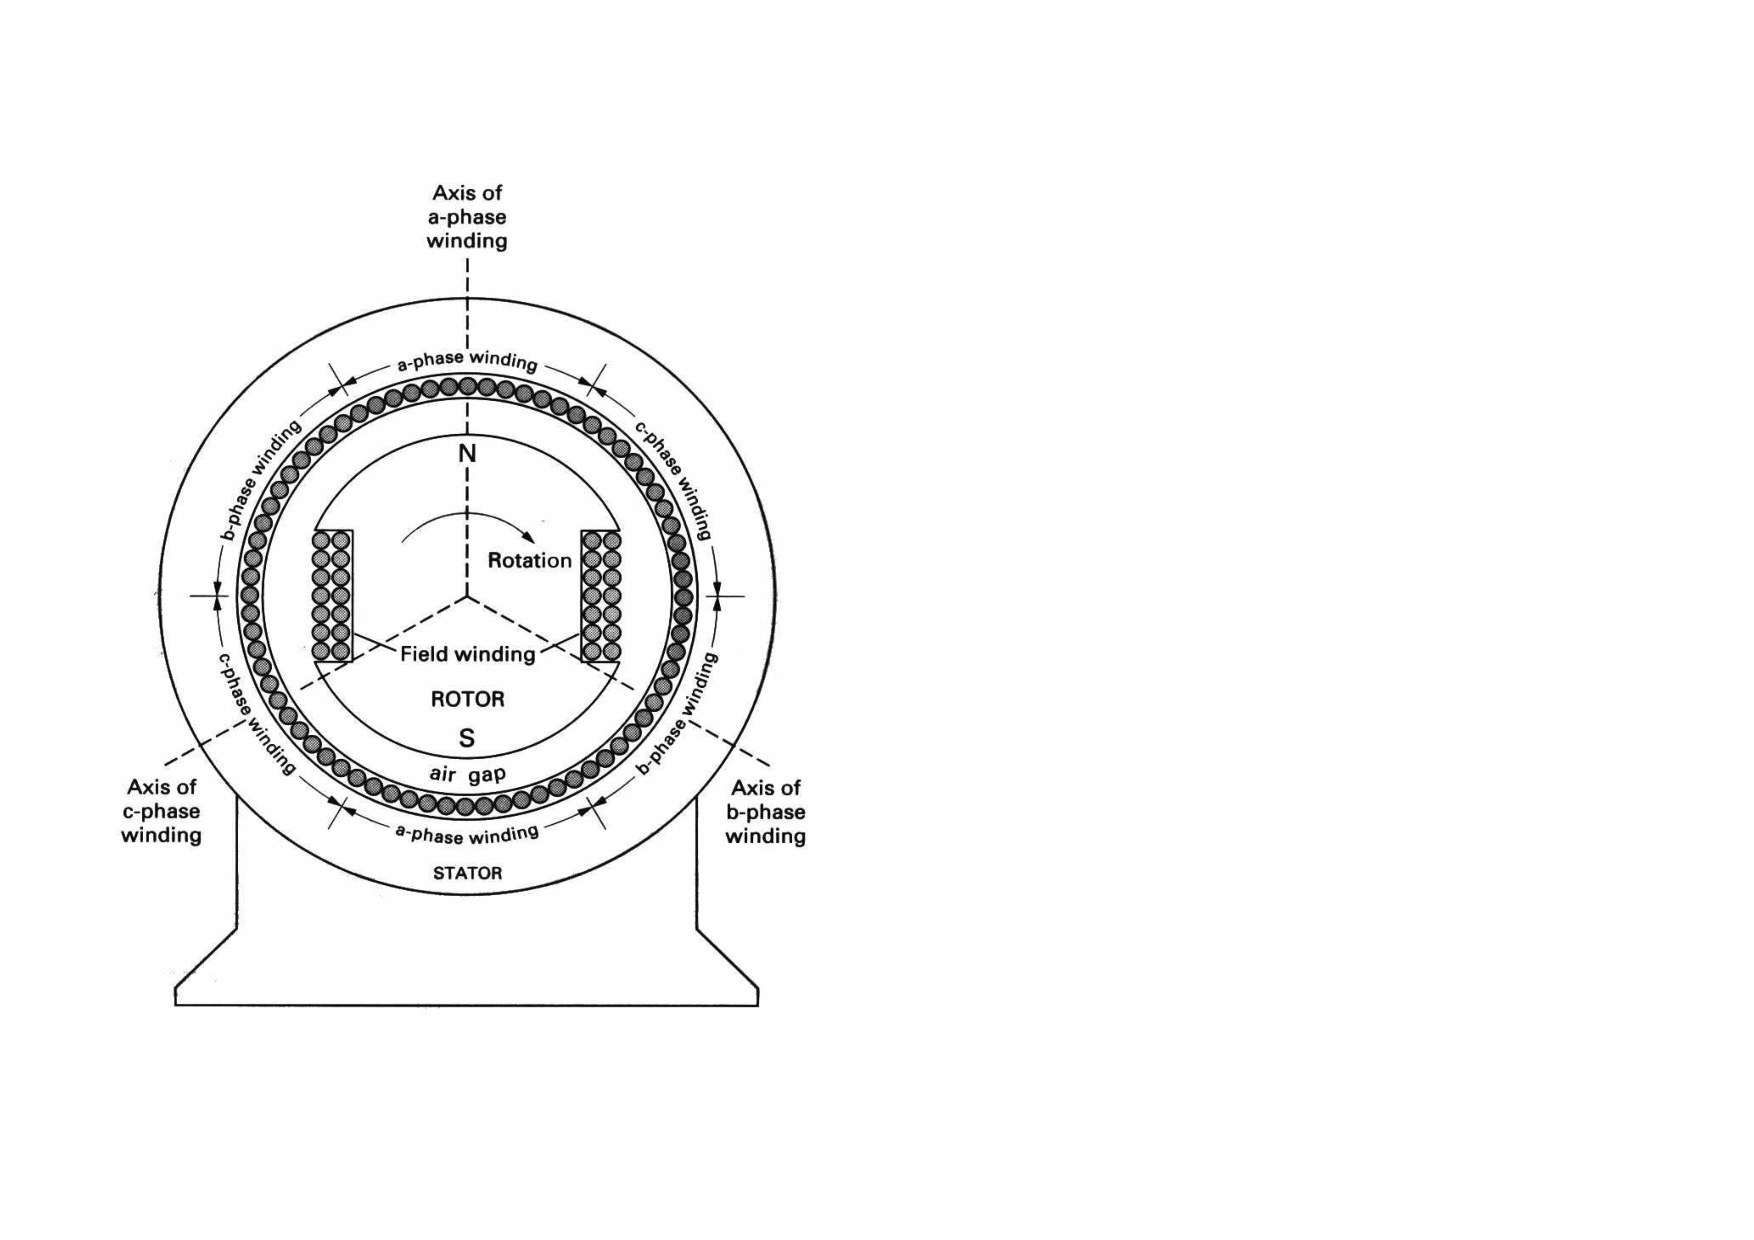
\includegraphics[width=0.8\linewidth]{3phase_gen}
		\end{center}
		\end{column}
		\begin{column}{0.5\linewidth}
			
			Le rotor tourne à une vitesse angulaire constante $\omega$.
			
			Pour les réseaux à 50 Hz : 3000 tours/min (Rem :  la vitesse peut être divisée
			par un facteur p si le rotor possède plusieurs paires de pôles).
			
			Circuit d'excitation du rotor parcouru par un courant continu. 
			
			Génère des f.e.m. égales en amplitude mais déphasées temporellement
			d'un tiers de période (correspond à un déphasage de 120$^{\circ}$).
		\end{column}
	\end{columns}
\end{frame}


\begin{frame}{Tensions et courants triphasés équilibrés}
	
	Si le système est équilibré, tous les courants et tensions
	correspondants dans les 3 phases sont égaux en amplitude et décalés
	temporellement d'un tiers de période = tensions et courants triphasés équilibrés.
	
	\begin{columns}
		\begin{column}{0.3\linewidth}
		\begin{center}
			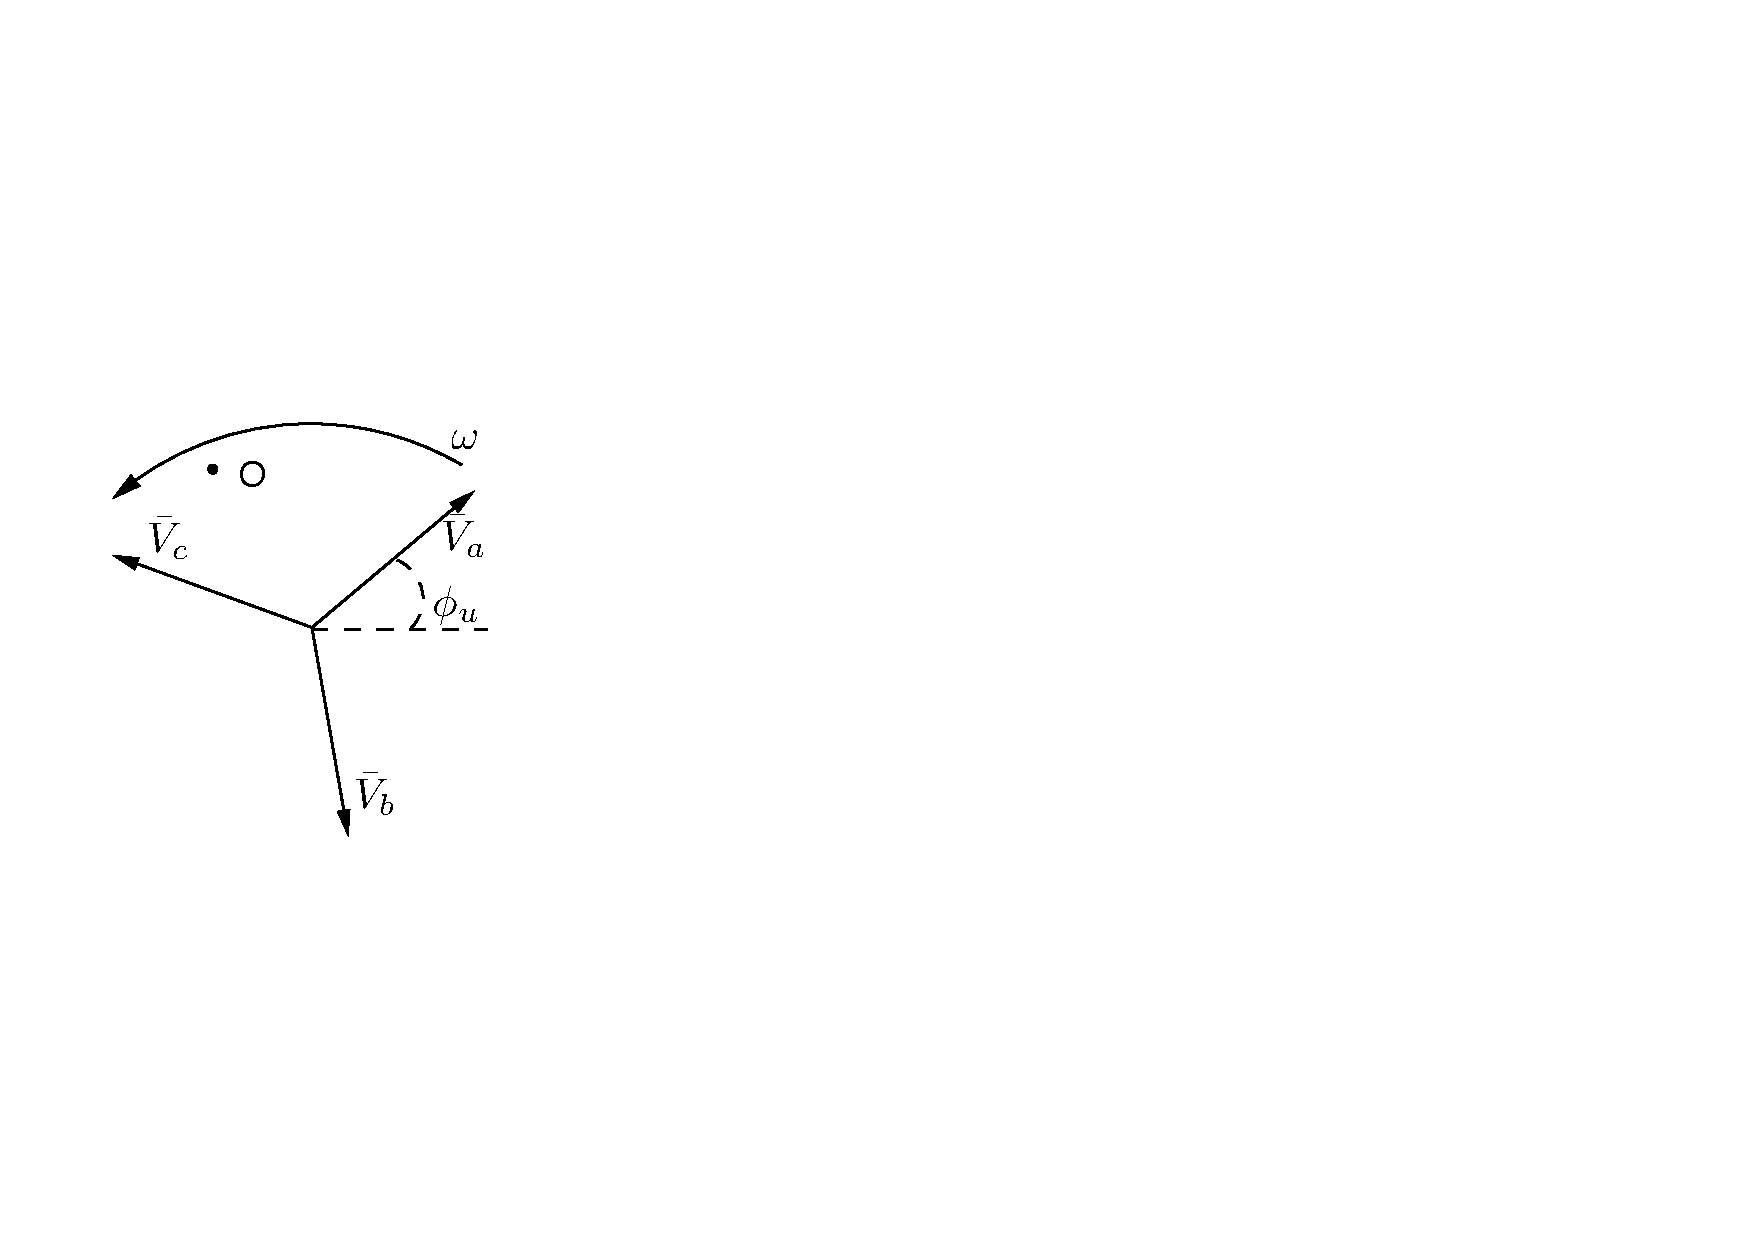
\includegraphics[width=0.8\linewidth]{3phase_U}
		\end{center}
		\end{column}
		\begin{column}{0.7\linewidth}
			{\small \begin{alignat*}{2}
				\bar{V}_a& =  Ve^{j\phi_u} & \quad v_a(t) & =\sqrt{2}V\cos(\omega t+\phi_u)\\
				\bar{V}_b& =  Ve^{j(\phi_u-\frac{2\pi}{3})} &  \quad v_b(t) &
				=\sqrt{2}V\cos(\omega t+\phi_u-\frac{2\pi}{3})\\
				& = \bar{V}_ae^{-j\frac{2\pi}{3}} & & = \sqrt{2}V\cos(\omega (t-\frac{T}{3})+\phi_u)\\
				\bar{V}_c& =  Ve^{j(\phi_u-\frac{4\pi}{3})} & \quad v_c(t) & 
				=\sqrt{2}V\cos(\omega t+\phi_u-\frac{4\pi}{3}) \\
				& = \bar{V}_ae^{-j\frac{4\pi}{3}}& & = \sqrt{2}V\cos(\omega (t-\frac{2T}{3})+\phi_u)
				\end{alignat*}}
		\end{column}
	\end{columns}
	

	Séquence directe des 3 phases a,b,c : observateur placé en O voit
	passer les vecteurs tournants dans l'ordre a,b,c.
	
	Autre sens = séquence inverse. 
\end{frame}


\begin{frame}{}
\begin{columns}
	\begin{column}{0.3\linewidth}
		\begin{center}
			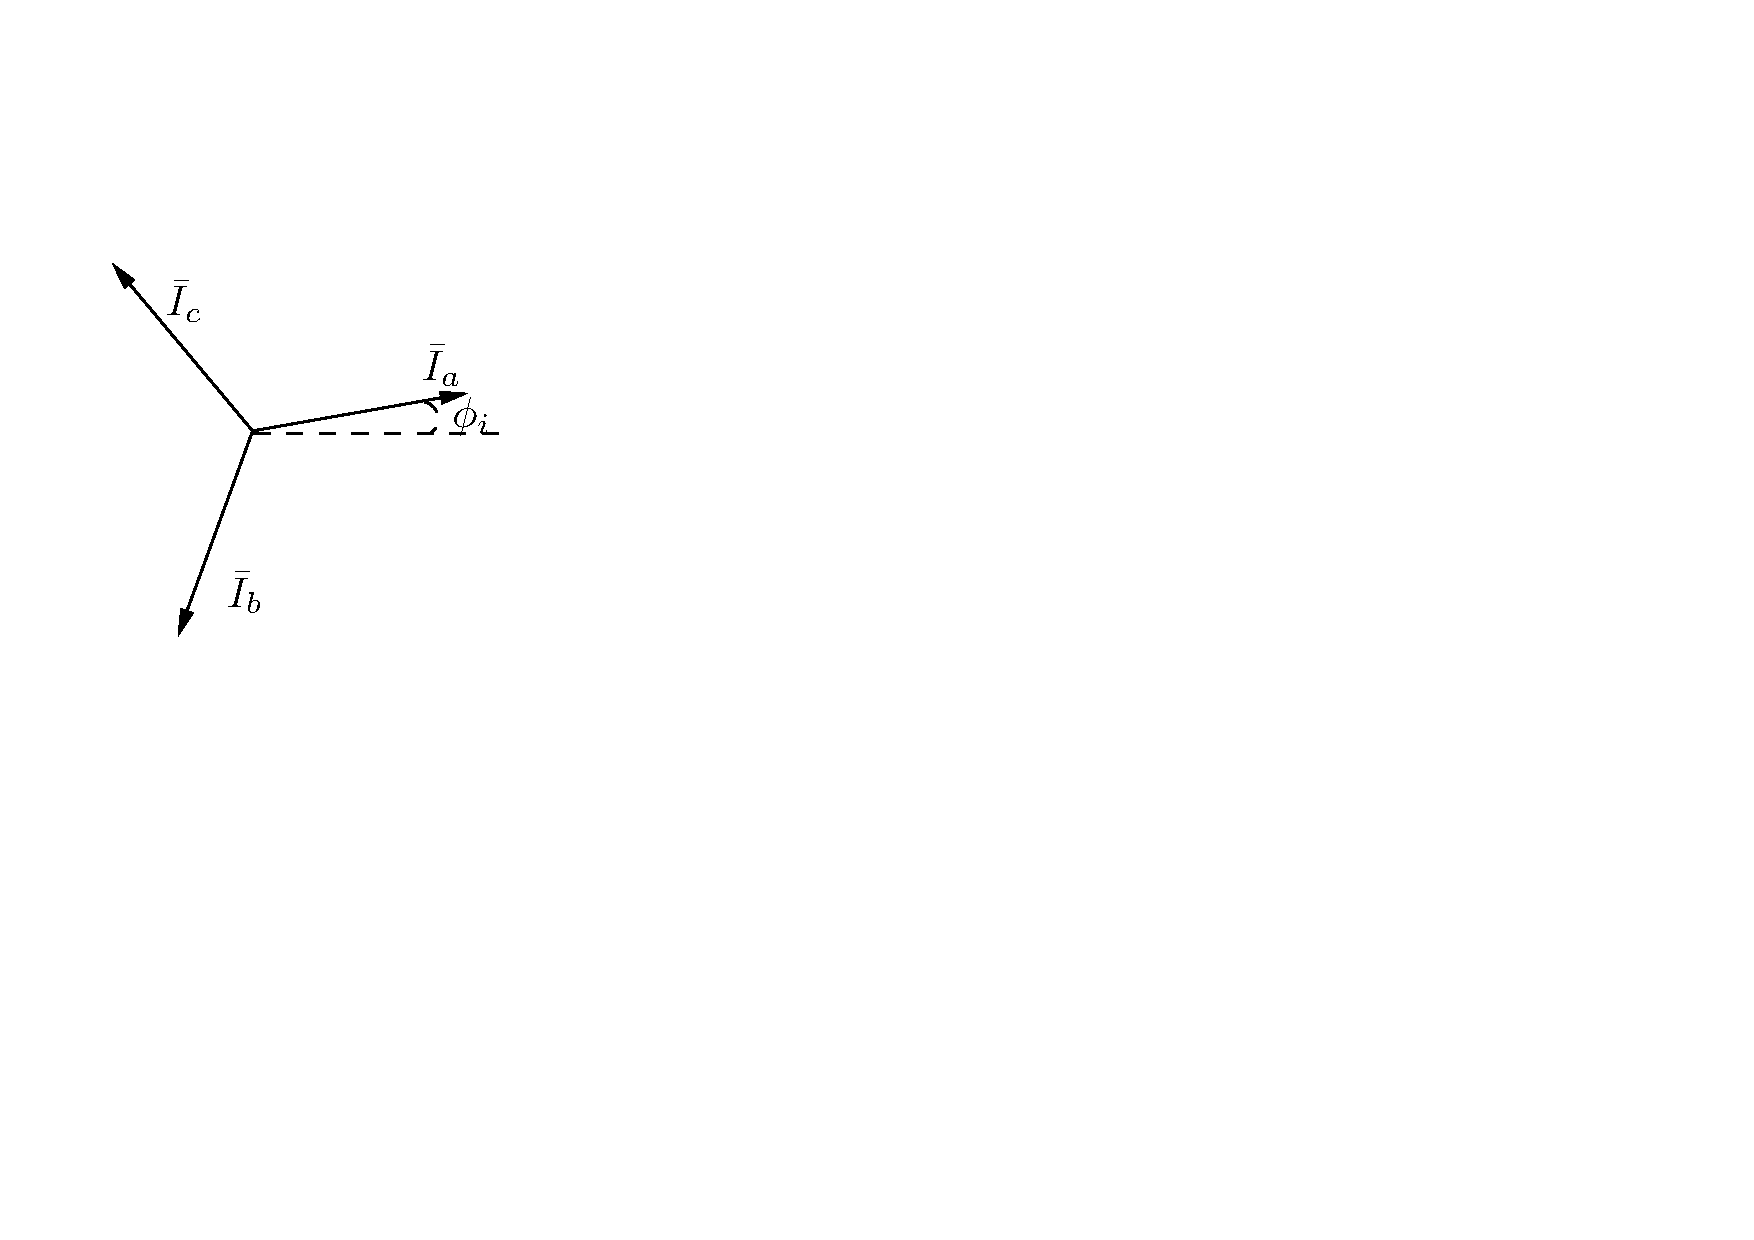
\includegraphics[width=0.8\linewidth]{3phase_I}
		\end{center}
	\end{column}
	\begin{column}{0.7\linewidth}
		{\small \begin{alignat*}{2}
			\bar{I}_a& =  Ie^{j\phi_i} & \quad i_a(t) & =\sqrt{2}I\cos(\omega t+\phi_i)\\
			\bar{I}_b& =  Ie^{j(\phi_i-\frac{2\pi}{3})} &  \quad i_b(t) &
			=\sqrt{2}I\cos(\omega t+\phi_i-\frac{2\pi}{3})\\
			& = \bar{I}_ae^{-j\frac{2\pi}{3}} & & = \sqrt{2}I\cos(\omega (t-\frac{T}{3})+\phi_i)\\
			\bar{I}_c& =  Ie^{j(\phi_i-\frac{4\pi}{3})} & \quad i_c(t) & 
			=\sqrt{2}I\cos(\omega t+\phi_i-\frac{4\pi}{3}) \\
			& = \bar{I}_ae^{-j\frac{4\pi}{3}}& & = \sqrt{2}I\cos(\omega (t-\frac{2T}{3})+\phi_i)
			\end{alignat*}}
	\end{column}
\end{columns}
	
	On a :
	\[\bar{V}_a+\bar{V}_b+\bar{V}_c=0\]
	\[\bar{I}_a+\bar{I}_b+\bar{I}_c=0\]
\end{frame}

\subsection{Montage en étoile}
\begin{frame}{Montage en étoile}
	\begin{center}
	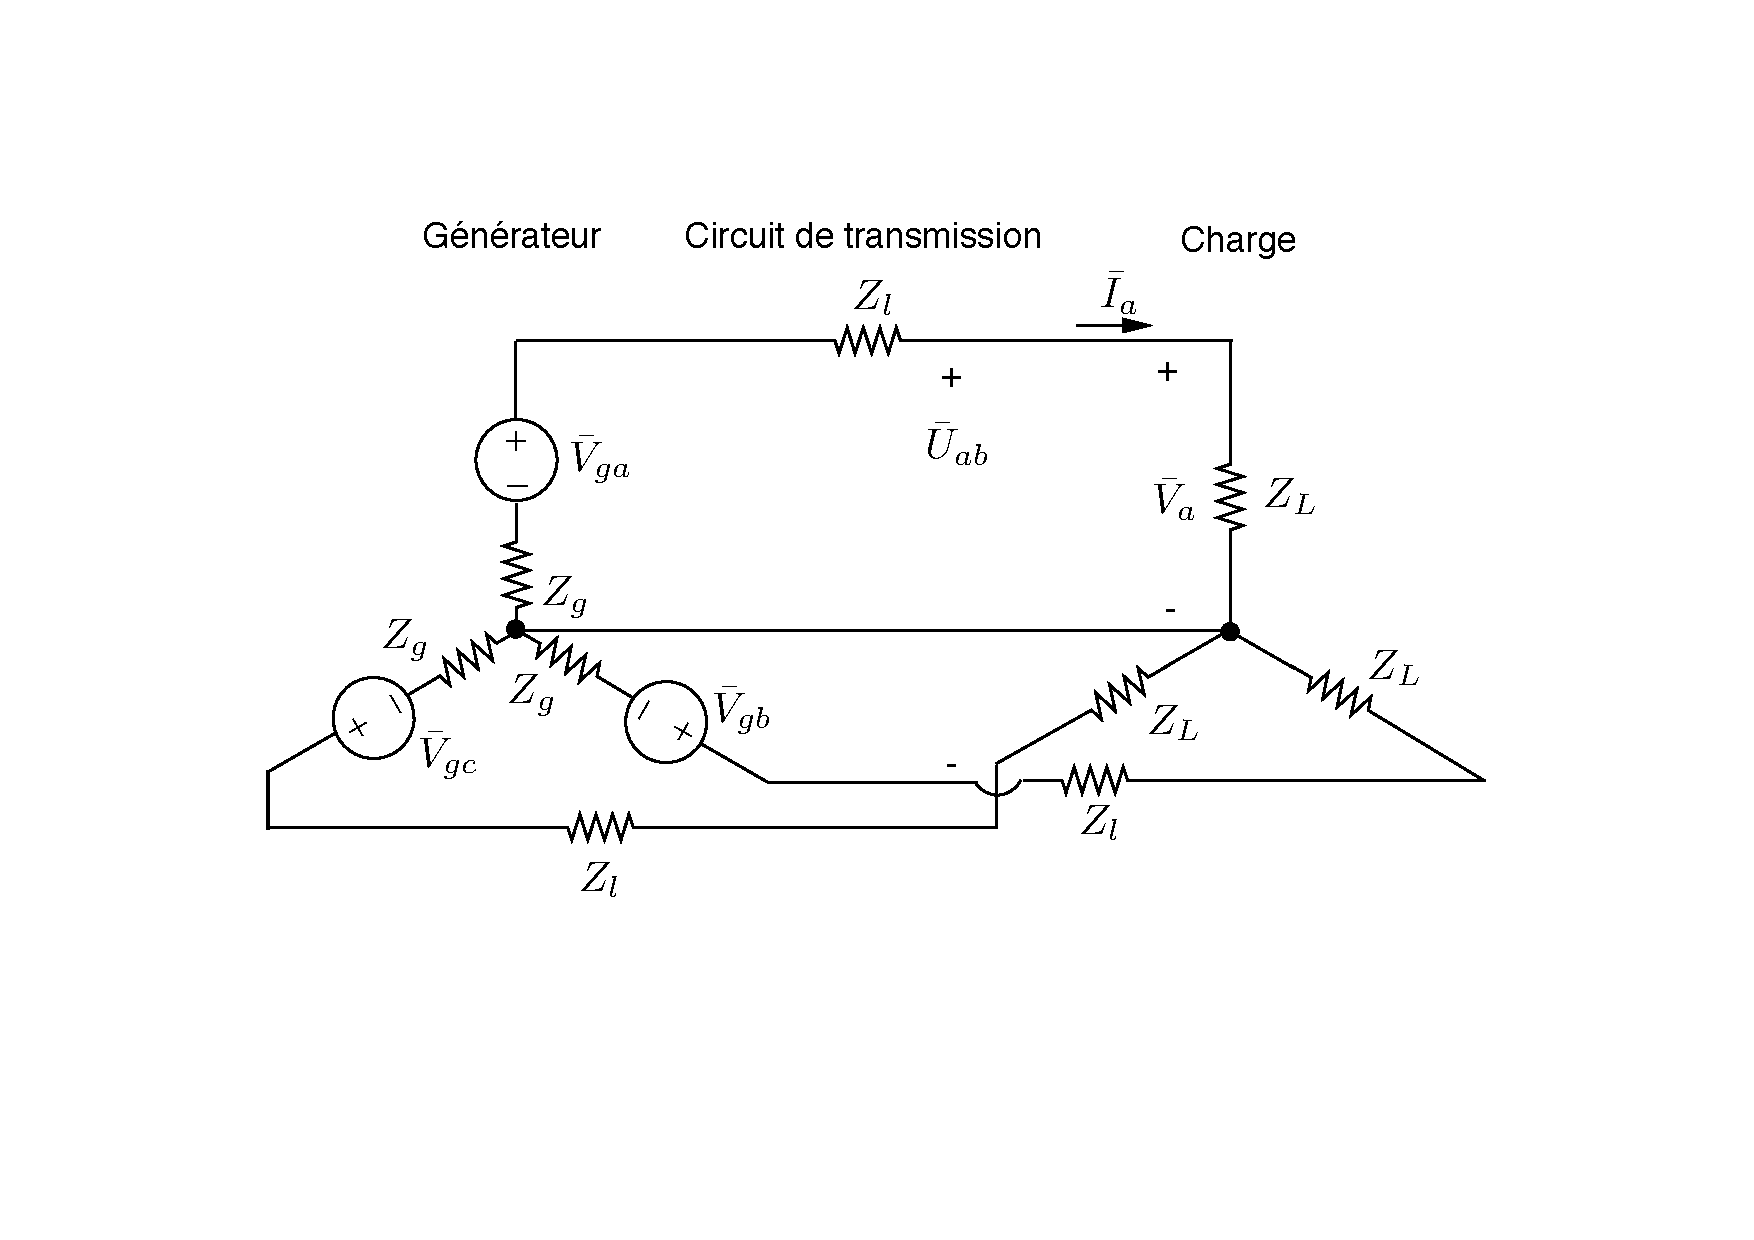
\includegraphics[width=.8\linewidth]{principe_3phase}
	\end{center}
	
	Le courant dans le conducteur  reliant les {\em neutres  N et
		N$^{'}$}  est :
	\[\bar{I}_a+\bar{I}_b+\bar{I}_c=0\]
	
	En régime parfaitement équilibré, tous les neutres sont au même potentiel.
\end{frame}

\begin{frame}{Tension de phase et tension de ligne}
	
	$\bar{V}_a$ est une {\bf tension de phase} (ou tension simple) : c'est
	la différence de potentiel aux bornes d'une charge monophasée, ou la
	différence de potentiel entre une ligne et le neutre.
	
	\vfill
	$\bar{U}_{ab}$ est une {\bf tension de ligne} (ou tension composée ou
	tension entre phases) : c'est la différence de potentiel entre deux
	phases.
\end{frame}


\begin{frame}{Les trois tensions de ligne sont}
\begin{columns}
	\begin{column}{6cm}
		\begin{eqnarray*}
			\bar{U}_{ab}& =&
			\bar{V}_a-\bar{V}_b=\sqrt{3}\bar{V}_ae^{j\frac{\pi}{6}}\\
			\bar{U}_{bc}& =& \bar{V}_b-\bar{V}_c=\sqrt{3}\bar{V}_be^{j\frac{\pi}{6}}\\
			\bar{U}_{ca}& =& \bar{V}_c-\bar{V}_a=\sqrt{3}\bar{V}_ce^{j\frac{\pi}{6}}\
		\end{eqnarray*}
	\end{column}
	\begin{column}{6cm}
	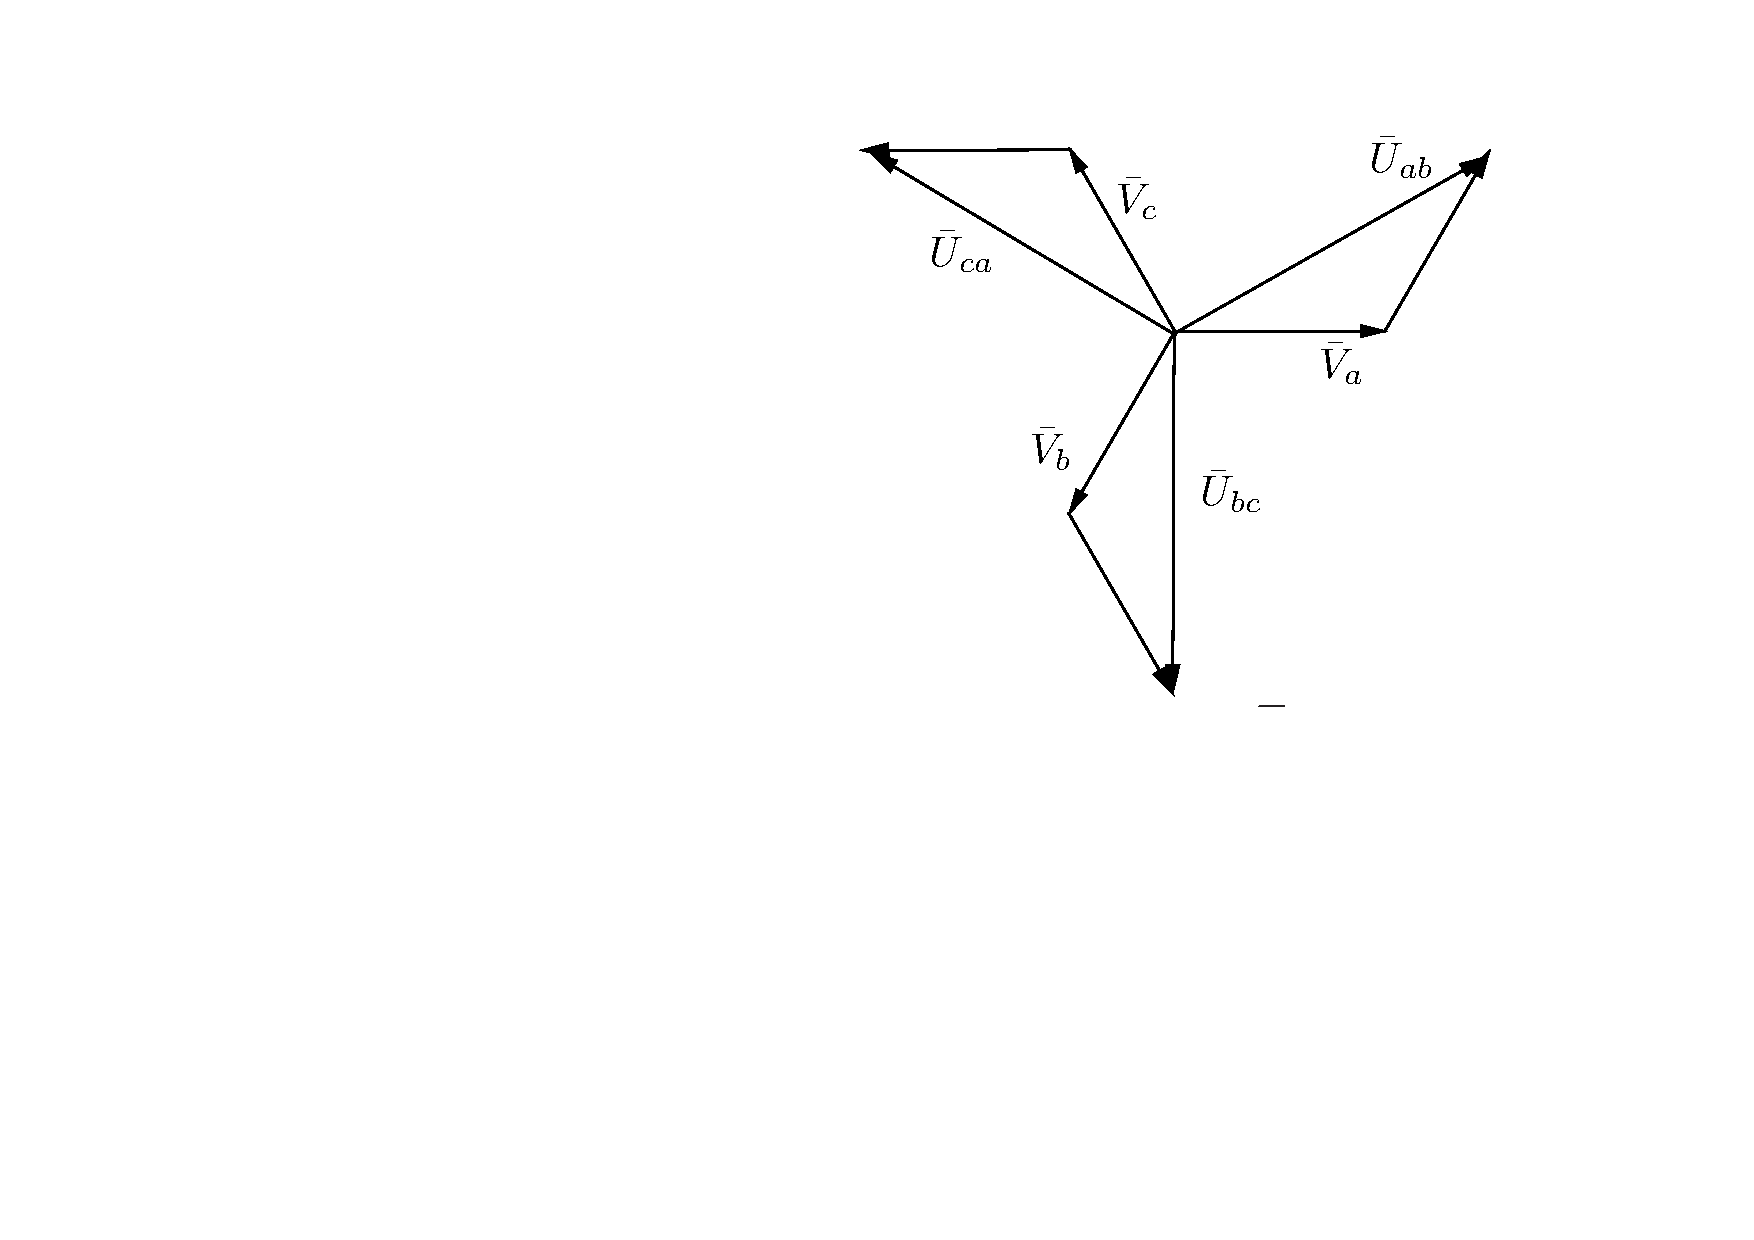
\includegraphics[width=0.7\linewidth]{3phase_tension_de_ligne}
	\end{column}
\end{columns}

$\bar{U}_{ab}$, $\bar{U}_{bc}$, $\bar{U}_{ca}$ forment aussi une
séquence directe et
$U=\sqrt{3}V$

Dans un montage en étoile, on dispose de deux tensions.

Distribution domestique :
\begin{itemize}
	\item tension de phase : 220 V (tension phase-neutre)
	\item tension de ligne : 380 V
\end{itemize}
\end{frame}


\begin{frame}{Mise à la terre des  neutres}
	
	En régime équilibré, le courant dans le conducteur de neutre est nul
	$\rightarrow$ on peut supprimer ce conducteur.
	\begin{center}
	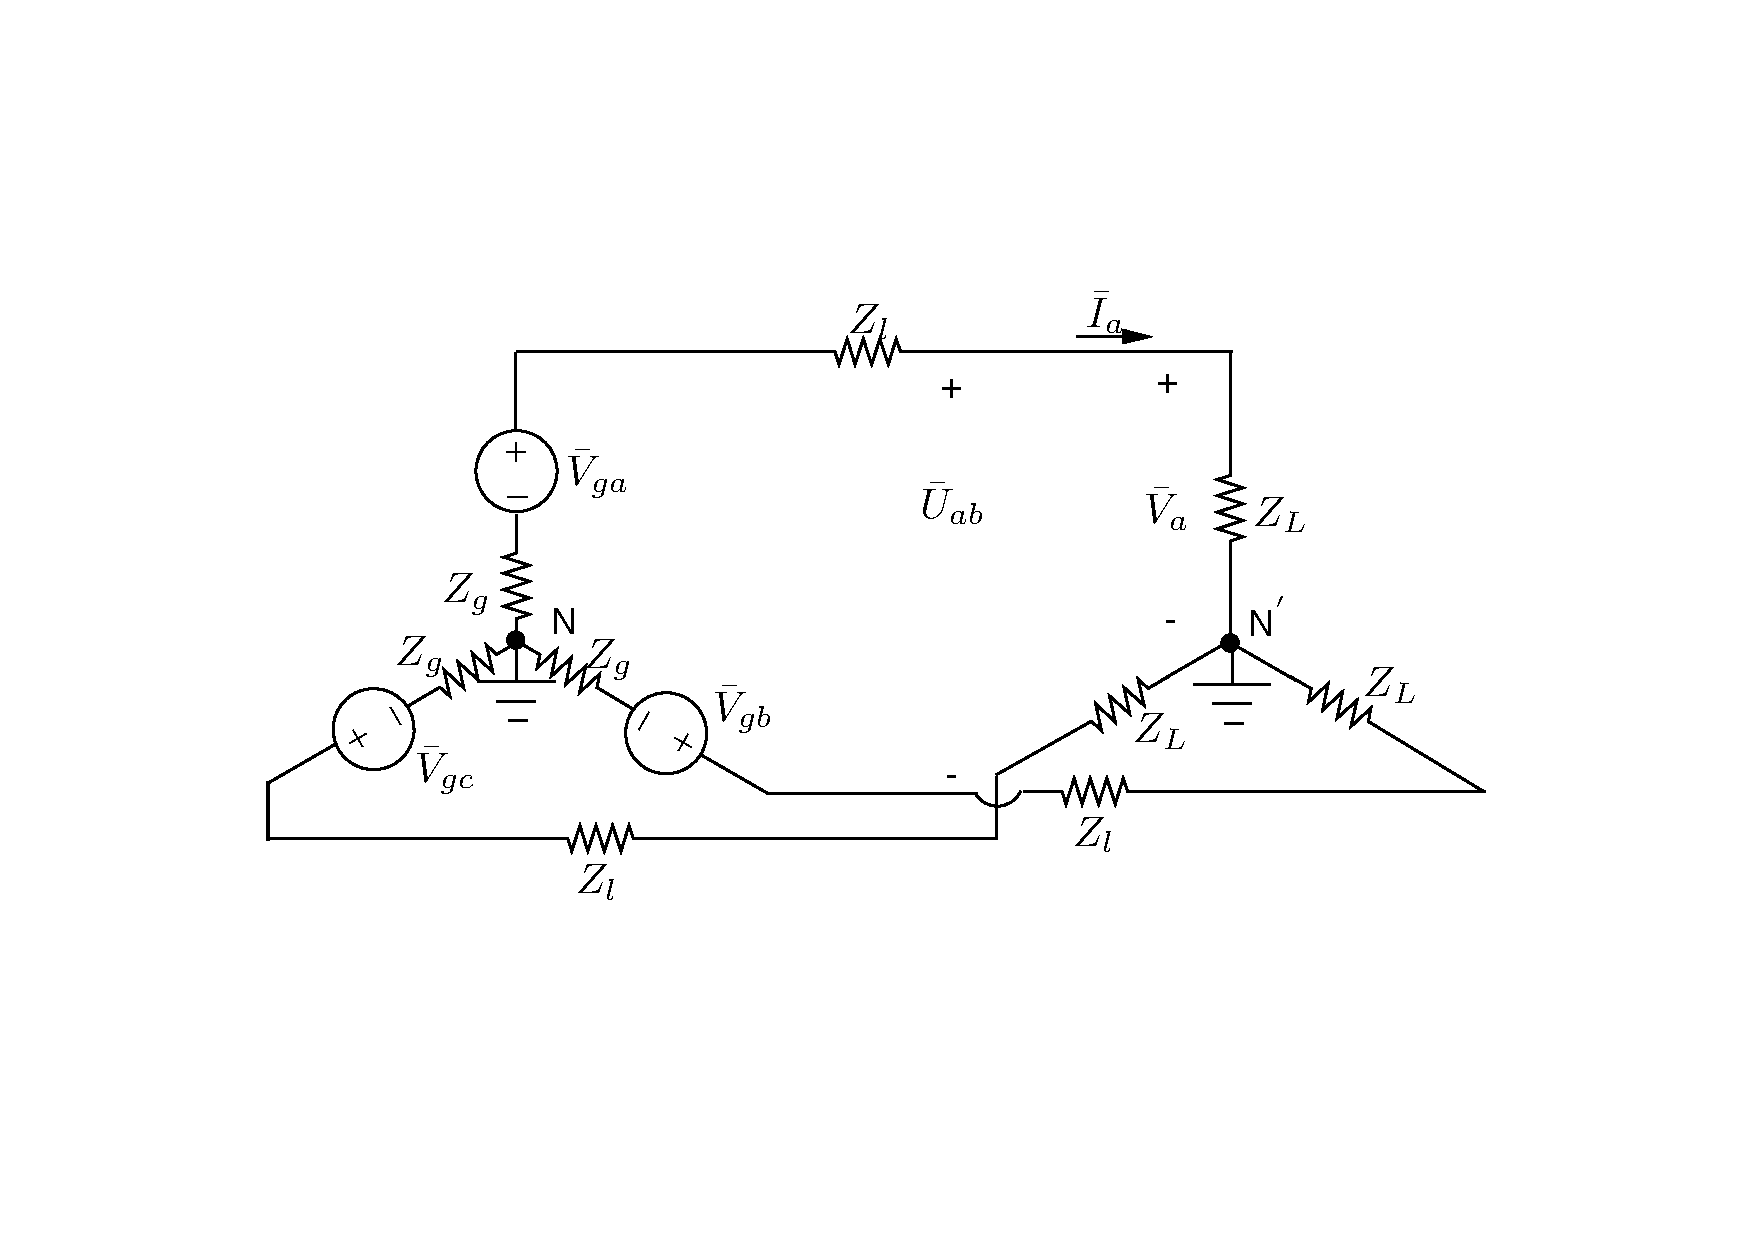
\includegraphics[width=0.7\linewidth]{3phase_grounding}	
	\end{center}
	
	En pratique, il existe toujours un léger déséquilibre entre les
	phases et on connecte les neutres à la terre. 
\end{frame}

\begin{frame}{Avantages}
	\begin{itemize}
		\item faible courant de déséquilibre  circule via la terre
		\item en cas de court-circuit entre une phase et la terre, évite les surtensions : \\
		soit $\bar{V}_c=0$, 
		\begin{itemize}
			\item si N et N$^{'}$ ne sont pas mis à la terre,
			différences de potentiel entre les deux autres phases et la terre =
			tension composée = $\sqrt{3}V$, tension supérieure à la tension
			normale;
			\item si N et N$^{'}$ sont mis à la terre:\
			\begin{itemize}
			\item différences de
			potentiel entre les deux autres phases et la terre conservent des
			valeurs normales,
			\item courant de "fuite" $i_a+i_b+i_c$ non
			négligeable circule via la terre entre le point de court-circuit et
			le neutre, 
			\item ce courant peut être détecté par une protection (disjoncteur différentiel !) \\
		\end{itemize}
		\end{itemize}
	\end{itemize}
\end{frame}


\subsection{Connexion en triangle}
\begin{frame}{Connexion en triangle}
	Un équipement triphasé peut être connecté en étoile comme plus haut ou
	en triangle.
	
	\begin{columns}
		\begin{column}{0.4\linewidth}
			\flushright
			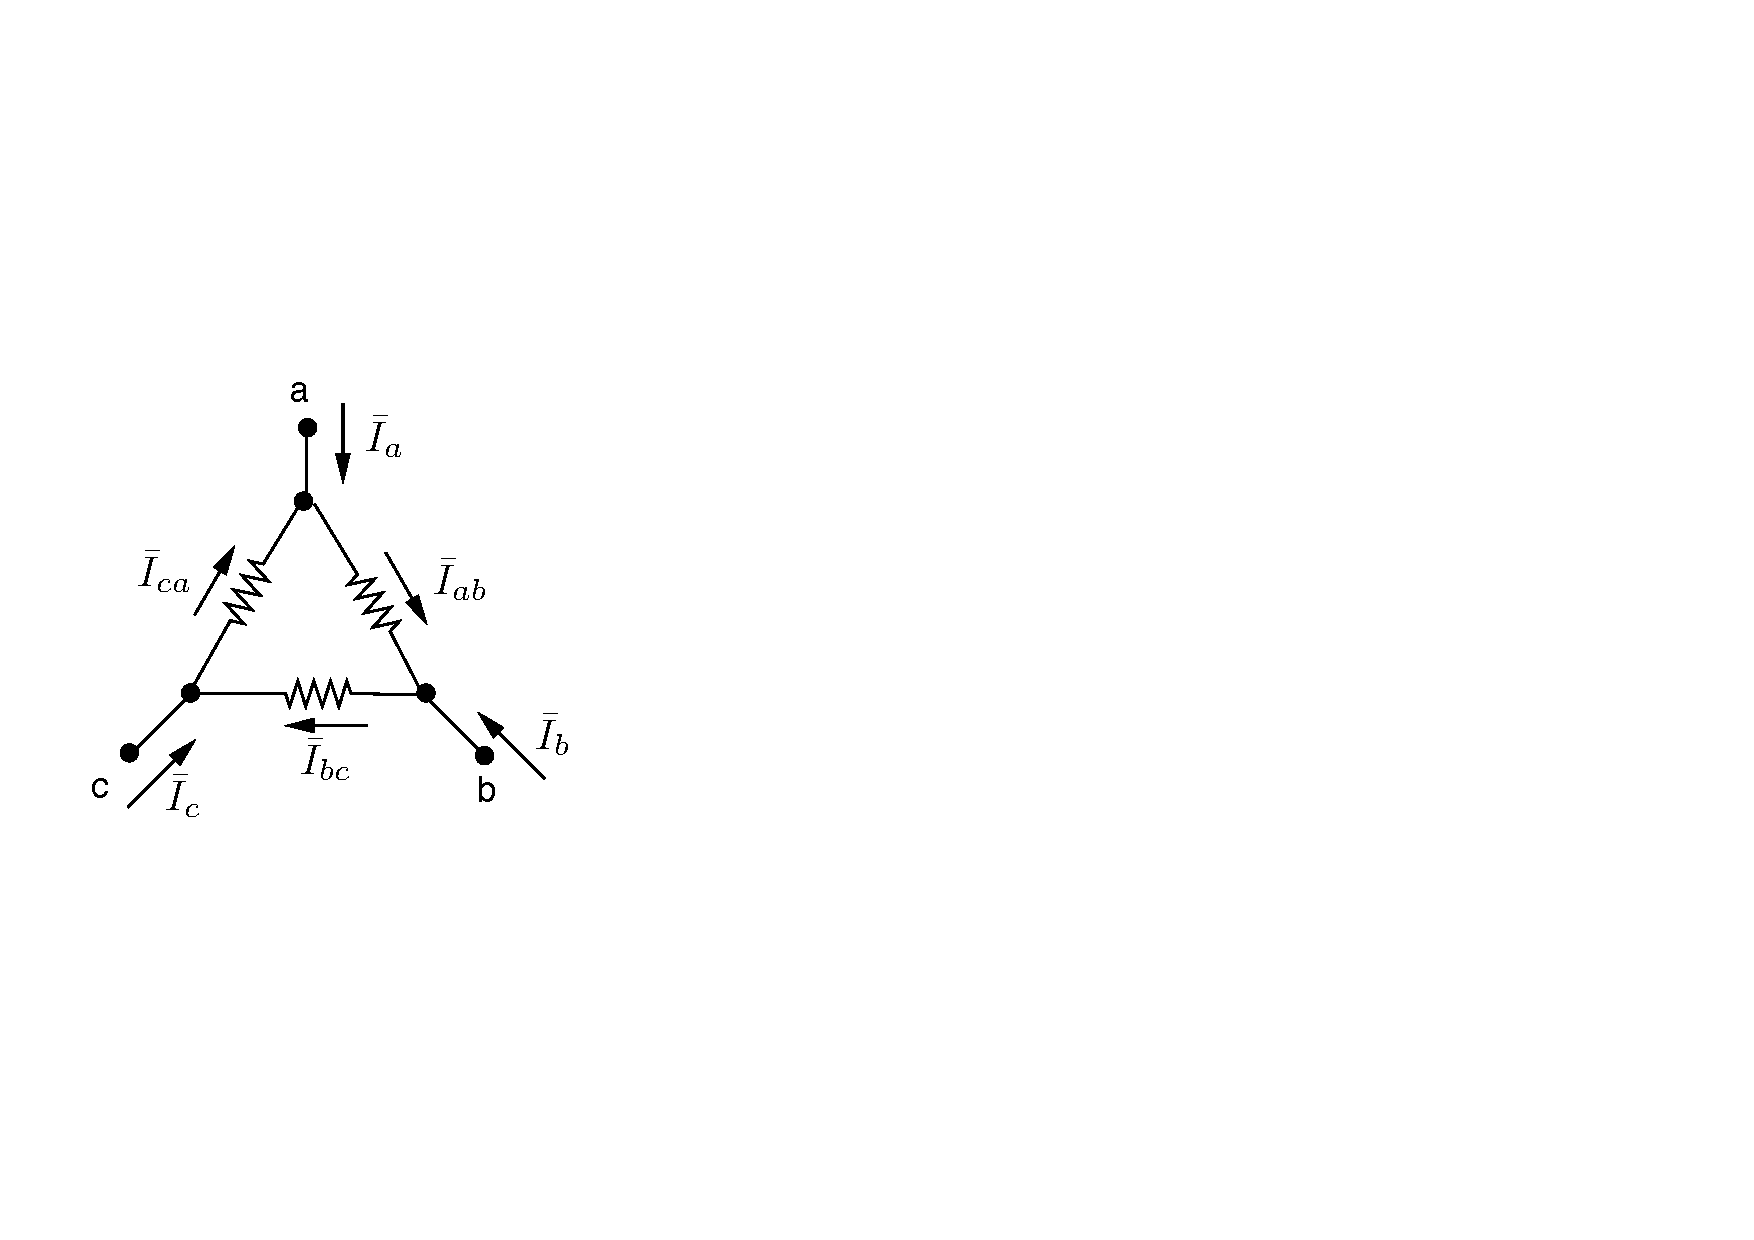
\includegraphics[width=0.7\linewidth]{3phase_triangle}	
		\end{column}
		\begin{column}{0.6\linewidth}
			Une seule tension, la tension de ligne,  mais  deux courants.
			
			Pas de point neutre.
		\end{column}
	\end{columns}
	
	$\bar{I}_a$, $\bar{I}_b$, $\bar{I}_c$ sont les courants de ligne\\
	$\bar{I}_{ab}$, $\bar{I}_{bc}$, $\bar{I}_{ca}$ sont les courants de phase
\end{frame}


\begin{frame}{}
	\begin{columns}
		\begin{column}{0.5\linewidth}
			\begin{eqnarray*}
				\bar{I}_{a}& =&
				\bar{I}_{ab}-\bar{I}_{ca}=\sqrt{3}\bar{I}_{ab}e^{-j\frac{\pi}{6}}\\
				\bar{I}_{b}& =& \bar{I}_{bc}-\bar{I}_{ab}=\sqrt{3}\bar{I}_{bc}e^{-j\frac{\pi}{6}}\\
				\bar{I}_{c}& =& \bar{I}_{ca}-\bar{I}_{bc}=\sqrt{3}\bar{I}_{ca}e^{-j\frac{\pi}{6}}\
			\end{eqnarray*}
		\end{column}
		\begin{column}{0.5\linewidth}
			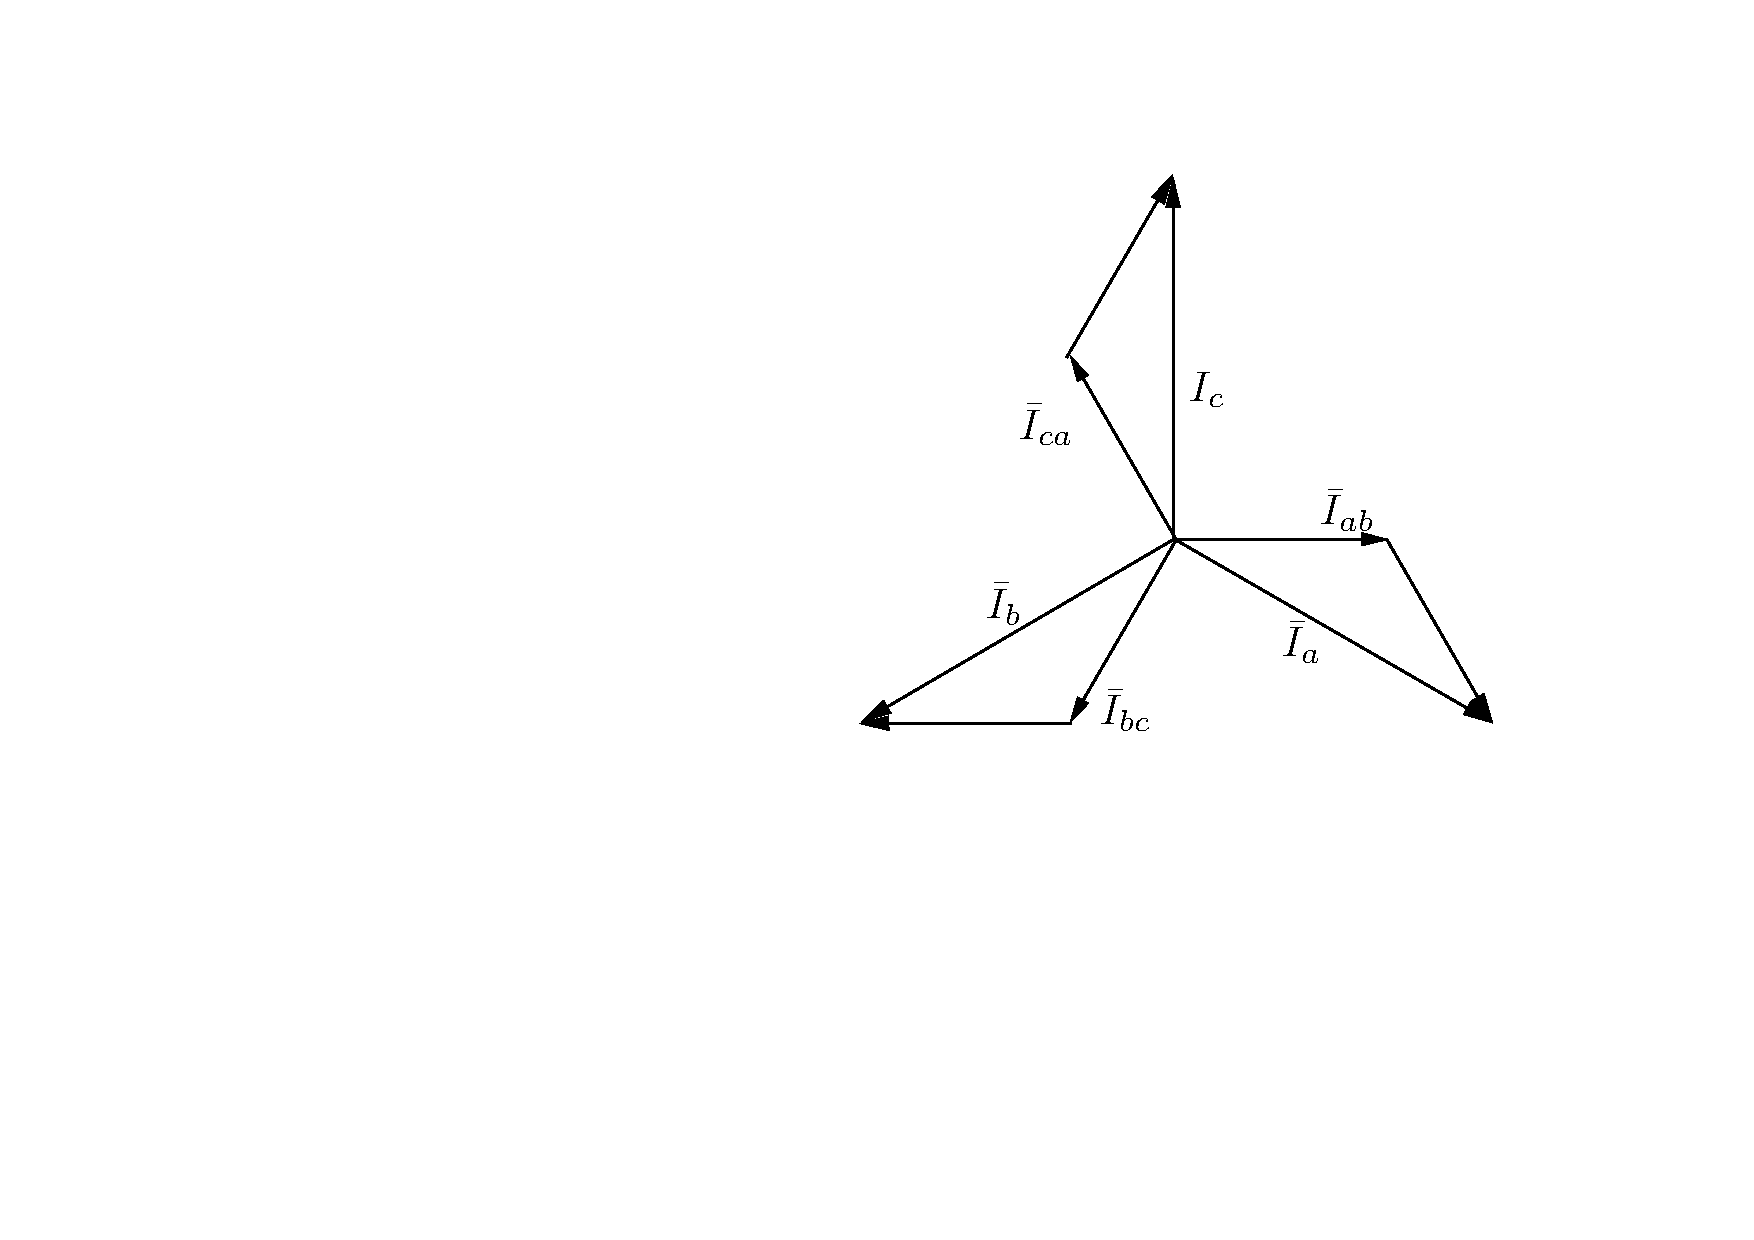
\includegraphics[width=0.7\linewidth]{3phase_power_star}	
		\end{column}
	\end{columns}
	
	Soit $I_l$ l'amplitude des courants de ligne et $I_{ph}$ l'amplitude
	des courants de phase :
	\[I_l=\sqrt{3}I_{ph}\]
\end{frame}


\subsection{Puissances}
\begin{frame}{Montage étoile}
	
	Puissance instantanée fournie à une charge triphasée connectée en
	étoile :
	{\small \begin{eqnarray*}
			p_{3\phi}(t)& =& v_ai_a+v_bi_b+v_ci_c\\
			& = & 2VI\left[\cos(\omega t+\phi_u)\cos(\omega t+\phi_i)+ \right.\\
			& & \left. + \cos(\omega
			t+\phi_u-\frac{2\pi}{3})\cos(\omega t+\phi_i-\frac{2\pi}{3})+ \right.\\
			& & \left. +\cos(\omega t+\phi_u-\frac{4\pi}{3})\cos(\omega
			t+\phi_i-\frac{4\pi}{3})\right]\\
			& = &3VI\cos(\phi_u-\phi_i)+ VI\left[
			\cos(2\omega t+\phi_u+\phi_i)+ \right.\\
			& & \left. + \cos(2\omega t+\phi_u+\phi_i-\frac{2\pi}{3})+
			\cos(2\omega t+\phi_u+\phi_i-\frac{4\pi}{3})\right]\\
			& = & 3VI\cos(\phi_u-\phi_i)=3P
		\end{eqnarray*}}
		$p_{3\phi}(t)$ est constante !\\
		$p_{3\phi}(t)$ = 3 x la P active consommée par l'impédance $Z_L$  d'une des phases.
\end{frame}
	
	%------------------------------------------------------------------------

\begin{frame}{}
	Puissance complexe triphasée fournie à une charge triphasée connectée en
	étoile~:
	{\small \begin{eqnarray*}
			S_{3\phi}& = &\bar{V}_a\bar{I}_a^*+\bar{V}_b\bar{I}_b^*+\bar{V}_c\bar{I}_c^*\\
			& = & \bar{V}_a\bar{I}_a^*(1+e^{-j\frac{2\pi}{3}}e^{j\frac{2\pi}{3}}+
			e^{-j\frac{4\pi}{3}}e^{j\frac{4\pi}{3}})\\
			& =& 3\bar{V}_a\bar{I}_a^*\\
			& = & 3VI(\cos(\phi_u-\phi_i)+j\sin(\phi_u-\phi_i))
		\end{eqnarray*}}
		Puissance active triphasée :
		\[P_{3\phi}=3VI\cos(\phi_u-\phi_i)\]
		Puissance réactive triphasée :
		\[Q_{3\phi}=3VI\sin(\phi_u-\phi_i)\]
		
		$Q_{3\phi}$ : notion artificielle puisque $p_f$ triphasée =0 !
		
		Seule $Q$ par phase a une signification physique.
\end{frame}
		
		%------------------------------------------------------------------------
		
\begin{frame}{Montage triangle}
	
	Puissance instantanée fournie à une charge triphasée connectée en
	triangle :
	{\small \begin{eqnarray*}
		p_{3\phi}(t)& =& u_{ab}i_{ab}+u_{bc}i_{bc}+u_{ca}i_{ca}\\
		& = & 3UI_{ph}\cos(\phi_u-\phi_i)=3P
	\end{eqnarray*}}
	Puissance complexe triphasée fournie à une charge triphasée connectée en
	triangle~:
	
	\begin{columns}
		\begin{column}{4cm}
			\flushright
			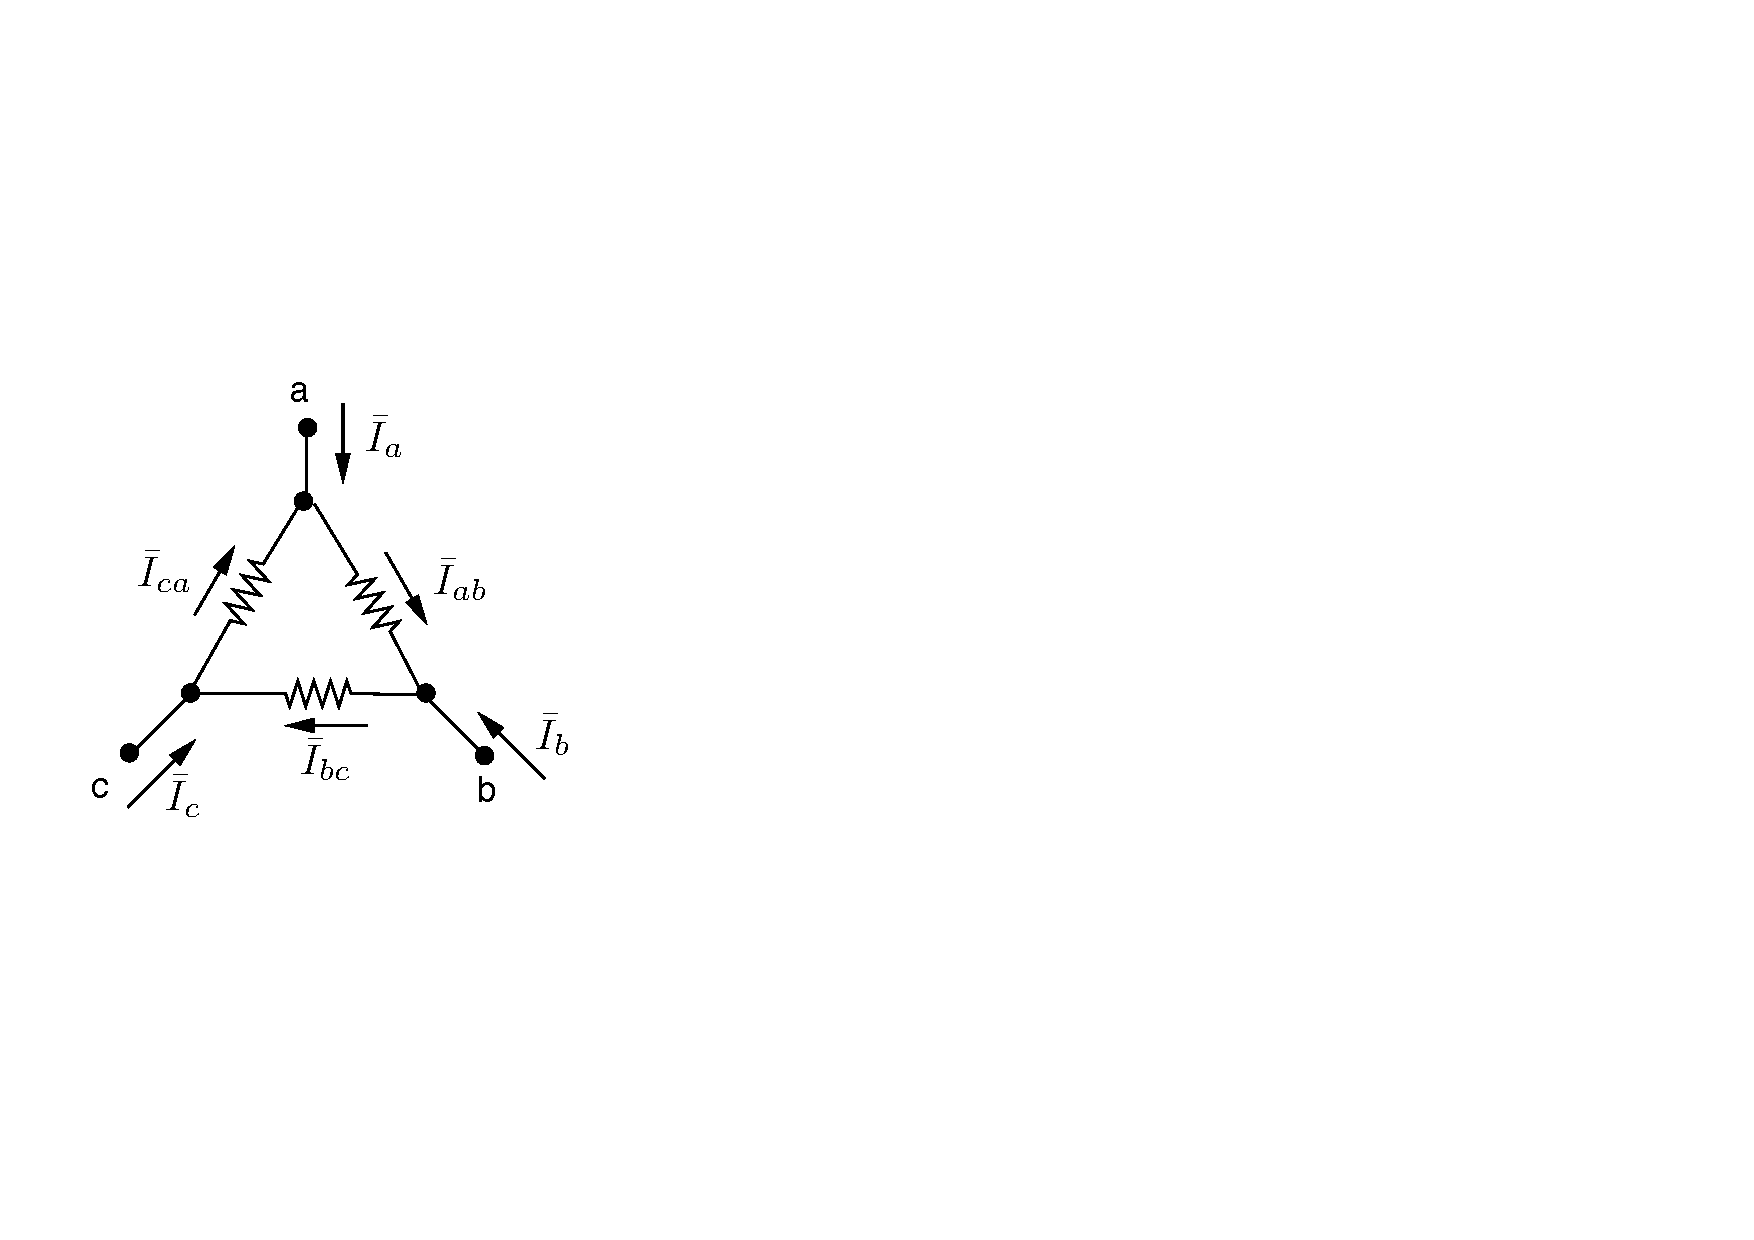
\includegraphics[width=0.7\linewidth]{3phase_triangle}	
		\end{column}
		\begin{column}{8cm}
			{\small \begin{eqnarray*}
					S_{3\phi}& = &\bar{U}_{ab}\bar{I}_{ab}^*+\bar{U}_{bc}\bar{I}_{bc}^*+\bar{U}_{ca}\bar{I}_{ca}^*\\
					& = & 3UI_{ph}(\cos(\phi_u-\phi_i)+j\sin(\phi_u-\phi_i))\\
					& =& P_{3\phi}+jQ_{3\phi}
				\end{eqnarray*}}
		\end{column}
	\end{columns}
\end{frame}
		
				%------------------------------------------------------------------------

\begin{frame}{}
	Etoile :
	{\small \begin{eqnarray*}
			P_{3\phi}& =& 3VI\cos(\phi_u-\phi_i)= \sqrt{3}UI\cos(\phi_u-\phi_i)\\
			Q_{3\phi}& = & 3VI\sin(\phi_u-\phi_i)= \sqrt{3}UI\sin(\phi_u-\phi_i)
		\end{eqnarray*}}
		Triangle :
		{\small \begin{eqnarray*}
				P_{3\phi}& =& 3UI_{ph}\cos(\phi_u-\phi_i)= \sqrt{3}UI_{l}\cos(\phi_u-\phi_i)\\
				Q_{3\phi}& = & 3UI_{ph}\sin(\phi_u-\phi_i)= \sqrt{3}UI_{l}\sin(\phi_u-\phi_i)
			\end{eqnarray*}}
Pour les deux montages :
{\small \begin{eqnarray*}
		P_{3\phi}& =& \sqrt{3}UI\cos(\phi_u-\phi_i)\\
		Q_{3\phi}& = & \sqrt{3}UI\sin(\phi_u-\phi_i)\\
		p_{3\phi}(t)& = & P_{3\phi}=3P
	\end{eqnarray*}}
	\begin{itemize}
		\item $U$ est l'amplitude de la tension de ligne
		\item $I$ est l'amplitude du courant de ligne
		\item $\phi_u-\phi_i$ est le déphasage entre la tension de phase et le
		courant de phase
	\end{itemize}
\end{frame}


\begin{frame} {Circuits triphasés équilibrés}
	\begin{block}{Synthèse}
		\begin{itemize}
			\item Three-phase system: three conductors carrying currents by design shifted of $120^\circ$,  plus one neutral \item Hence 4 conductors in total instead of 2 in single-phase
			\item Line voltage $\bar{U}$ vs. phase voltage $\bar{V}$: $\bar{U}=\sqrt{3} \bar{V} e^{j \pi / 6}$			
			\item Instantaneous power is constant: $P=3VI \cos \phi  = \sqrt{3} UI cos \phi$!
			\item There is a fluctuating power in each phase!
			\item Why three-phase? Less conductors w.r.t carried power, less vibrations.
			\item Why \textit{balanced}? Simpler for analysis, desirable economically: neutral conductor can in theory be removed
		\end{itemize}
	\end{block}
\end{frame}

\end{document}
